\chapter{Simulations in MATLAB}\label{cha:sim_matlab}
Simulations are a powerful tool for evaluating the performance of multi-agent systems in various scenarios. In this chapter, we present the simulation of the system in MATLAB \citep{matlab_2022}, a widely-used platform for scientific computing and engineering applications. We develop a simulation framework that integrates the various components of the system, including path following, formation control, and obstacle avoidance, and demonstrate its effectiveness in a range of scenarios. The simulations provide insights into the system's behavior under different conditions and enable us to test and refine our control algorithms. 


The chapter is organized as follows. Section~\ref{sec:numerical_auv} details the numerical model used in the simulations. Section~\ref{sec:centralized_simulations} demonstrates the effectiveness of the centralized \gls{nsb} algorithm through three different simulation scenarios. Section~\ref{sec:distributed_simulations} demonstrates the effectiveness of the distributed \gls{nsb} algorithm, first through a general experiment with collision avoidance, formation keeping, and path following, and then through three comparison studies with the first-order distributed method from \cite{matous_formation_2023}, the hand-position-based consensus method from \cite{restrepo_tracking--formation_2022}, and the alternative distributed formulation from Section~\ref{sec:alternative_distributed}.

\section{Numerical AUV model}\label{sec:numerical_auv}
We chose the \gls{lauv}, shown in Figure~\ref{fig:lauv}, as the vehicle model for simulation \citep{sousa_lauv_2012}. The plant model in our simulation environment is set up to exactly match our ideal model \eqref{eq:auv_model}. That means there are no modeling errors, and the fleet should behave as expected from theory. This section details the derivation of the numerical model used in the simulation.

\begin{figure}[htb]
    \centering
    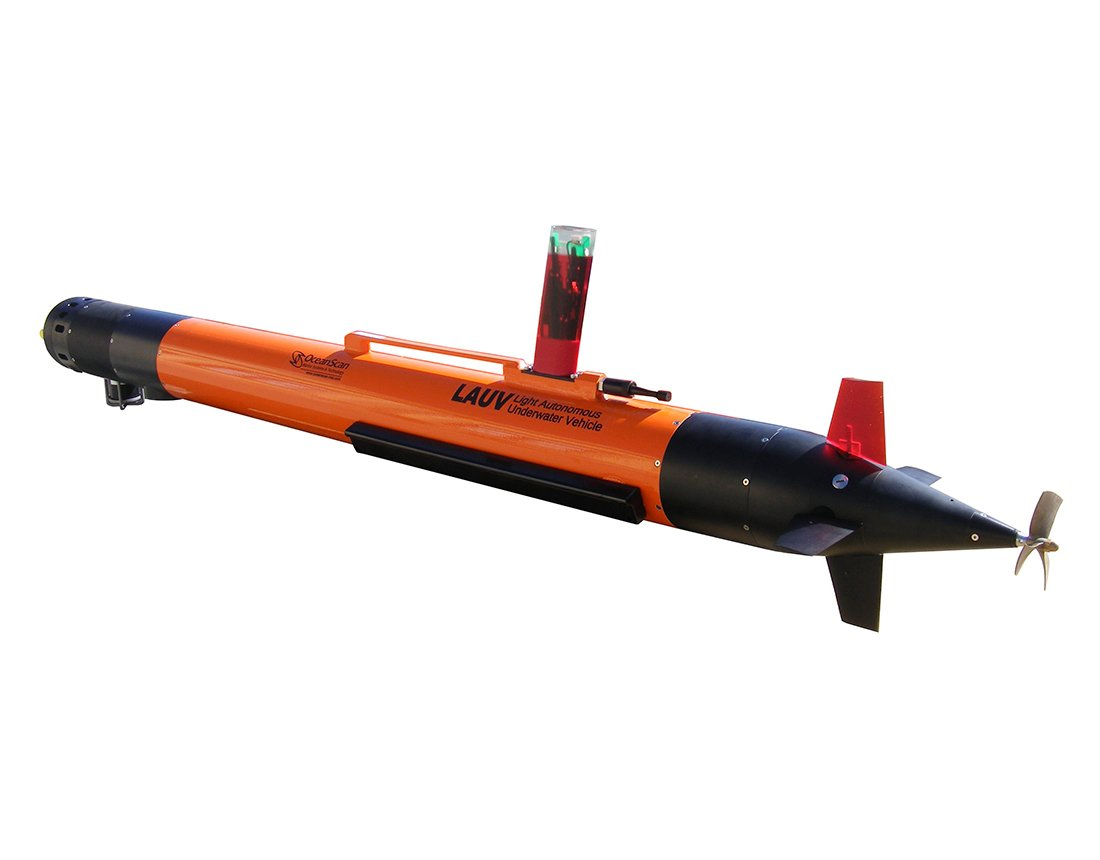
\includegraphics[width=.7\textwidth, trim={0cm 8.1cm 0cm 8cm}, clip]{figures/lauv-square-00.jpg}
    \vspace{-2mm}
    \caption{The LAUV modeled in this simulation study. Image is taken from OceanScan website \citep{noauthor_lauv_nodate}.}
    \label{fig:lauv}
\end{figure}
\vspace{-2mm}
A model for the \gls{lauv} with the origin of the coordinate frame at the center of buoyancy is developed in \cite{estrela_da_silva_modeling_2007}. The modeling closely follows that of \cite[Section 8.4]{fossen_handbook_2021}. Following Assumption~\ref{assumption:three} from Chapter~\ref{cha:vehicle_model} we will develop the model around the pivot point (PP). We will first present a model with the origin at the center of buoyancy (CB) and then transform the model to the pivot point using the pivot point transformation \eqref{eq:pp_transform_matrix}. Following \cite{estrela_da_silva_modeling_2007} we consider a \gls{lauv} with a length $L = 104\, \mathrm{cm}$, a diameter $D = 15\, \mathrm{cm}$, a mass of $18\, \mathrm{kg}$ and distance between CB and center of gravity (CG) $z_g = 1\, \mathrm{cm}$.

The mass matrix $\mathbf{M} = \mathbf{M}_{RB} + \mathbf{M}_A$ consists of the rigid body mass matrix and the added mass matrix. The rigid body mass matrix is derived as a diagonal matrix in CG and transformed to CB
\begin{equation}
    \mathbf{M}_{RB}^{CB} = \mathbf{H}\T([0\,0\,z_g]\T) \mathrm{diag}([m\, m\, m\, I_x\, I_y \, I_z]) \mathbf{H}([0\,0\,z_g]\T),
\end{equation}
where $\mathbf{H}$ is a coordinate transformation matrix given in \cite[Appendix C]{fossen_handbook_2021}, $I_x = \tfrac{1}{10} m D^2$ and $I_y=I_z = \tfrac{1}{20}m (L^2+D^2)$. The added mass matrix is diagonal in CB because of symmetry, and the numerical calculation can be found in \cite[Section 8.4]{fossen_handbook_2021}. The resulting mass matrix with numerical values is given by
\begin{equation}\label{eq:M_CB}
    \mathbf{M}^{CB} = \begin{bmatrix}
19 & 0 & 0 & 0 & 0.18 & 0 \\
0 & 34 & 0 & -0.18 & 0 & 0 \\
0 & 0 & 34 & 0 & 0 & 0 \\
0 & -0.18 & 0 & 0.04 & 0 & 0 \\
0.18 & 0 & 0 & 0 & 1.8 & 0 \\
0 & 0 & 0 & 0 & 0 & 1.8
\end{bmatrix}.
\end{equation}
The corresponding damping matrix is taken from \cite{estrela_da_silva_modeling_2007}, and the non-linear part is neglected according to Assumption~\ref{assumption:four}:
\begin{equation}
\mathbf{D}^{CB}(\bm{\zeta}_r) =
\begin{bmatrix}
2.4 & 0 & 0 & 0 & 0 & 0 \\
0 & 23 & 0 & 0 & 0 & -11.5\\
0 & 0 & 23 & 0 & 11.5 & 0 \\
0 & 0 & 0 & 0.3 & 0 & 0 \\
0 & 0 & -3.1 & 0 & 9.7 & 0 \\
0 & 3.1 & 0 & 0 & 0 & 9.7
\end{bmatrix}.
\end{equation}
To derive the control-input matrix we consider fins with an $x$-position of $-0.455, \mathrm{m}$ relative to the vehicle's mass center. Then, each newton meter of torque produced corresponds to $2.2\, \mathrm{N}$ produced force, which results in the following control-input matrix:\enlargethispage*{\baselineskip}
\begin{equation}
\mathbf{B}^{CB} = \begin{bmatrix}
1.0 & 0 & 0 & 0 \\
0 & 0 & 0 & -2.2 \\
0 & 0 & 2.2 & 0 \\
0 & 1.0 & 0 & 0 \\
0 & 0 & 1.0 & 0 \\
0 & 0 & 0 & 1.0
\end{bmatrix}.
\end{equation}


At this point, we note that, as a result of non-zero $z_g$ implicitly violating the top-bottom symmetry assumption (Assumption~\ref{assumption:one}), $\mathbf{M}^{CB}$ from \eqref{eq:M_CB} violates the structure from \cite[Equation 4]{borhaug_straight_2007}. Therefore, it will not be possible to find a transformation that exactly satisfies Assumption~\ref{assumption:three}. A common modeling approach is to neglect the off-diagonal elements of $\mathbf{M}^{CB}$ as they are dominated by the other modes of the system. The resulting model matrices are then given by
\begin{subequations}
\begin{align}
    \mathbf{M} &= \mathbf{H}_{PP}\T \mathrm{diag}(\mathbf{M}^{CB}) \mathbf{H}_{PP},\\
    \mathbf{D}(\bm{\zeta}_r) &= \mathbf{H}_{PP}\T \mathbf{D}^{CB}(\bm{\zeta}_r)  \mathbf{H}_{PP},\\
    \mathbf{B} &= \mathbf{H}_{PP}\T \mathbf{B}^{CB},
\end{align}
\end{subequations}
where $\mathbf{H}_{PP}$ is the pivot-point transformation matrix given by \eqref{eq:pp_transform_matrix}.

The Coriolis and centripetal matrix $\mathbf{C}(\bm{\zeta}_r) = \mathbf{C}_{RB}(\bm{\zeta}_r) + \mathbf{C}_A(\bm{\zeta}_r)$ consists of a rigid body term and an added mass term. Following \cite[Section~10.3]{fossen_handbook_2021}, we carefully model the rigid-body Coriolis matrix independently of linear velocities so that the model correctly handles irrotational constant ocean currents. The resulting Coriolis matrices are given by
\begin{align}
    \mathbf{C}_{RB}(\bm{\zeta}_r) &= \mathbf{H}_{PP}\T \begin{bmatrix}
        \mathbf{S}(m\bm{\omega}) & \mathbf{0}_{3\times 3}\\
        \mathbf{0}_{3\times 3} & \mathbf{S}([I_x p\; I_y q\; I_z r]\T)
    \end{bmatrix}\mathbf{H}_{PP},\\
    \mathbf{C}_A(\bm{\zeta}_r) &= \begin{bmatrix}
        \mathbf{0}_{3\times 3} & - \mathbf{S}(\mathbf{A}_{11} \bm{\nu}_r + \mathbf{A}_{12}\bm{\omega})\\
        - \mathbf{S}(\mathbf{A}_{11} \bm{\nu}_r + \mathbf{A}_{12}\bm{\omega}) & - \mathbf{S}(\mathbf{A}_{21} \bm{\nu}_r + \mathbf{A}_{22}\bm{\omega})
    \end{bmatrix},
\end{align}
where 
\begin{equation}
    \mathbf{H}_{PP}\T\mathbf{M}_A\mathbf{H}_{PP} \coloneqq \begin{bmatrix}
        \mathbf{A}_{11} & \mathbf{A}_{12}\\\mathbf{A}_{21} & \mathbf{A}_{22}
    \end{bmatrix}.
\end{equation}

% An alternative approach is to try to come as close as possible to satisfying Assumption\ref{assumption:three} by applying a coordinate transformation in the $z$-direction in addition to the transformation in $x$-direction given by \eqref{eq:borhaug_transformation}. We let the vector from the PP to CB $r_{pb}^p$ be given by
% \begin{equation}
%     r_{pb}^p = [x_{bp}\, 0 \, z_{bp}]\T, \quad x_{bp} = \frac{m_{66} b_{24}}{m_{22}b_{64}}, \, z_{bp} = -\frac{m_{15}}{m_{22}}.
% \end{equation}
% The transformation $\mathbf{M}^{PP} = \mathbf{H}\T(r_{pb}^p)\mathbf{M}^{RB}\mathbf{H}(r_{pb}^p)$ and $\mathbf{B}^{PP} = \mathbf{H}\T(r_{pb}^p) \mathbf{B}^{CB}$ eliminates all sway acceleration from the actuators and leaves the have accelerations negligible:
% \begin{equation}
%     (\mathbf{M}^{PP})^{-1} \mathbf{B}^{PP} = \begin{bmatrix}
%         0.053 & 0 & -0.042 & 0\\
% 0 & 0 & 0 & 0\\
% 0.0006 & 0 & 0.0001 & 0\\
% 0 & 24 & 0 & -5.1\\
% -0.0052 & 0 & 9.9 & 0\\
% 0 & 0 & 0 & 9.9
%     \end{bmatrix}.
% \end{equation}
\section{Centralized NSB algorithm simulation results}\label{sec:centralized_simulations}
This section presents three different simulation experiments with the centralized second-order \gls{nsb} method from Chapter~\ref{cha:nsb_tasks}. Section~\ref{sec:general_three_agent} details a simulation experiment with three \glspl{auv} equipped with the centralized \gls{nsb} controller with the collision cones obstacle avoidance method detailed in Section~\ref{sec:collision_cones}. Section~\ref{sec:individual_obstacle} details a similar experiment but with obstacle avoidance implemented as an individual high-priority task for each vehicle as detailed in Section~\ref{sec:individual_colav}. Section~\ref{sec:harmonic_motion} demonstrates through simulation how the second-order \gls{nsb} algorithm enables us to specify the formation-keeping task as an interpretable spring-damper system. 


\subsection{General three-agent mission}\label{sec:general_three_agent}
This section presents a general simulation scenario that demonstrates the effectiveness of the complete system. The fleet consists of three vehicles equipped with the \gls{nsb} controller \eqref{eq:combined_control_action}, with the choice of integral action (Section~\ref{sec:integral_action}) to compensate for the unknown ocean current and the collision cones method (Section~\ref{sec:collision_cones}) to avoid obstacles. The fleet should follow a continuous spiral-shaped path while avoiding collision with a cylindrical-shaped obstacle with radius $10\, \mathrm{m}$ and base circle in the $xy-$plane and origin $[x, \, y] = [100,\, -10]$. In the rest of this section, all distances will be given in meters, and units are omitted for simplicity.

The prescribed path is given by the following spiral-equation
\begin{equation}
       \mathbf{p}_p(\xi) = \mathbf{p}_{p,0} + \bigl[\xi, -40 \cos(\tfrac{\pi}{100} \xi), 20 \sin(\tfrac{\pi}{100} \xi)\bigr]\T,
\end{equation}
where \begin{equation}
    \mathbf{p}_{p,0} = \bigl[ 0, -40, 35 \bigr]\T.
\end{equation}
The barycenter relative formation is given by
\begin{equation}\label{eq:desired_formation_sim}
    \mathbf{p}_{f,1:3}^f = \begin{bmatrix}0 & 0 & 0 \\ 10 & -10 & 0 \\ 5 & 5 & -10\end{bmatrix},% \quad \mathbf{p}_{f,1}^f = \begin{bmatrix}0 \\ -10 \\ 5\end{bmatrix},\quad \mathbf{p}_{f,1}^f = \begin{bmatrix}0 \\ 0 \\ -10\end{bmatrix},
\end{equation}
and the collision avoidance task is configured to ensure a safe distance of $10\, \mathrm{m}$ both between vehicles in the fleet and external obstacles. Because the cylinder radius is $10\, \mathrm{m}$, its avoidance radius, $r_o$, is $20\, \mathrm{m}$. The activation angle $\alpha_{\min}$ is chosen as $15^\circ$. The vehicles are subject to an unknown ocean current 
\begin{equation}
    \mathbf{v}_c = \begin{bmatrix}
        0 & 0.25 & 0.05
    \end{bmatrix}\T \,\mathrm{m/s}.
\end{equation}

The controller gain matrices $\bm{\Lambda}_{p,1}$, $\bm{\Lambda}_{d,1}$, $\bm{\Lambda}_{p,2}$, $\bm{\Lambda}_{d,2}$, $\bm{\Lambda}_{p,3}$, and $\bm{\Lambda}_{i,3}$ from \eqref{eq:SOCLIK1}, \eqref{eq:saturated_formation_keeping}, and \eqref{eq:LOS_integral_controller} are chosen as scaled identity matrices $k_i \mathbb{I}$. The gains, as well as controller parameters $v_{2_{\max}}$, $\Delta_0$, $U_{LOS}$, and $k_\xi$ from \eqref{eq:saturated_formation_keeping} ,  \eqref{eq:error-dependent-lookahead}, \eqref{eq:desired_LOS}, and \eqref{eq:path_update}, and the hand length $h$ are given by Table~\ref{tab:simulation_parameters1}. The hand length is chosen as $5\, \mathrm{m}$ following \cite{matous_trajectory_2023} where the same \gls{auv} was simulated.

\begin{table}[ht]
  \centering
  \caption{Controller parameters used in simulation}
  \label{tab:simulation_parameters1}
  \begin{tabular}{ll}
    \hline
    Parameter & Value \\
    \hline
    $k_{p,1}$ & 1 \\
    $k_{d,1}$ & 0.2 \\
    $k_{p,2}$ & 0.5 \\
    $k_{d,2}$ & 1 \\
    $k_{p,3}$ & 1 \\
    $k_{i,3}$ & 1 \\
    $U_{LOS}$ & $1.5\, \mathrm{m/s}$ \\
    $\Delta_0$ & $5\, \mathrm{m}$ \\
    $k_\xi$ & 0.2 \\
    $v_{2_{\max}}$ & $0.75\, \mathrm{m/s}$ \\
    $h$ & $5 \, \mathrm{m}$\\
    \hline
  \end{tabular}
\end{table}

We initialize the fleet with barycenter $\mathbf{p}_b = [-5,\, -100,\, 18]\T$ and relative positions 
\begin{equation}
    \bm{\sigma}_{2,1:3} = \begin{bmatrix}0 & 0 & 0\\ -15 & 15 & 0 \\ -7 & -7 & 14\end{bmatrix}.% \quad \bm{\sigma}_{2,2} = \begin{bmatrix}0 \\ 15 \\ -7\end{bmatrix}, \quad \bm{\sigma}_{2,3} = \begin{bmatrix}0 \\ 0 \\ 14\end{bmatrix}.
\end{equation}

\begin{figure}[ht]
    \centering
    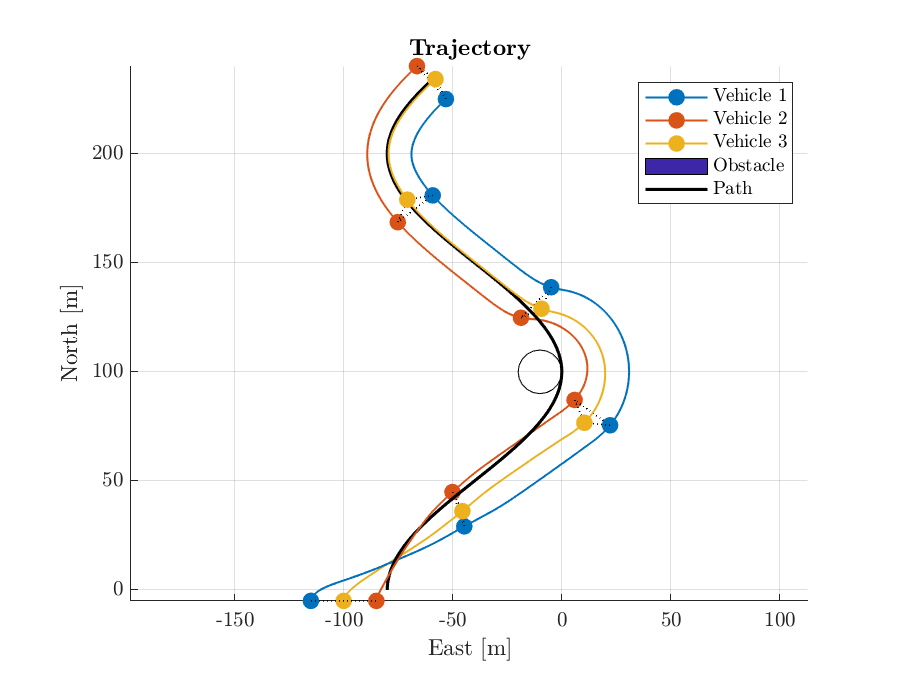
\includegraphics[width=.8\textwidth]{figures/sim-three-agent-general/plot3d-trajectory.eps}
    \vspace*{-4mm}
    \caption{The trajectory of the vehicles. The markers represent the vehicle positions every 50 seconds.}
    \label{fig:plot3d-general-mission}
    \vspace{-4mm}
\end{figure}


\begin{figure}[htbp]
    \centering
    \begin{subfigure}[t]{.9\textwidth}
    \centering
    \setlength\figurewidth{.8\linewidth}
    \setlength\figureheight{3cm}
    % This file was created by matlab2tikz.
%
%The latest updates can be retrieved from
%  http://www.mathworks.com/matlabcentral/fileexchange/22022-matlab2tikz-matlab2tikz
%where you can also make suggestions and rate matlab2tikz.
%
\definecolor{mycolor1}{rgb}{0.00000,0.44700,0.74100}%
\definecolor{mycolor2}{rgb}{0.85000,0.32500,0.09800}%
%
\begin{tikzpicture}

\begin{axis}[%
width=0.951\figurewidth,
height=\figureheight,
at={(0\figurewidth,0\figureheight)},
scale only axis,
xmin=0,
xmax=250,
xlabel style={at={(axis description cs:0.5,-0.08)}, font=\color{white!15!black}},
xlabel={Time [s]},
ymin=0,
ymax=25,
ylabel style={font=\color{white!15!black}, yshift=2mm},
ylabel={Distance [m]},
axis background/.style={fill=white},
every axis plot/.append style={line width=0.7pt},
title style={font=\bfseries, yshift=-2.75mm},
title={Smallest distances},
legend style={at={(0.97,0.02)}, anchor=south east, legend cell align=left, align=left, draw=white!15!black, legend columns=2,font=\footnotesize}
]
\addplot [color=mycolor1]
  table[]{collision_avoidance-1.tsv};
\addlegendentry{Inter-vehicle}

\addplot [color=mycolor2]
  table[]{collision_avoidance-2.tsv};
\addlegendentry{Obstacle}

\addplot[area legend, dashed, draw=black, fill=green, fill opacity=0.15, forget plot]
table[] {formation_keeping_error-10.tsv}--cycle;

\addplot [color=black, dashed]
  table[]{collision_avoidance-3.tsv};
\addlegendentry{$d_{\rm COLAV}$}


\addplot[area legend, dashed, draw=black, fill=white!50!red, fill opacity=0.25, forget plot]
table[] {collision_avoidance-4.tsv}--cycle;
\end{axis}
\end{tikzpicture}%
    \vspace*{-2mm}
    \caption{The minimum inter-vehicle and obstacle distance.}
    \label{fig:collision_avoidance}
    \end{subfigure}
    \\
    \begin{subfigure}[t]{.9\textwidth}
    \centering
    \setlength\figurewidth{.8\linewidth}
    \setlength\figureheight{3.3cm}
    % This file was created by matlab2tikz.
%
%The latest updates can be retrieved from
%  http://www.mathworks.com/matlabcentral/fileexchange/22022-matlab2tikz-matlab2tikz
%where you can also make suggestions and rate matlab2tikz.
%
\definecolor{mycolor1}{rgb}{0.00000,0.44700,0.74100}%
\definecolor{mycolor2}{rgb}{0.85000,0.32500,0.09800}%
\definecolor{mycolor3}{rgb}{0.92900,0.69400,0.12500}%
%
\begin{tikzpicture}

\begin{axis}[%
width=0.951\figurewidth,
height=\figureheight,
at={(0\figurewidth,0\figureheight)},
scale only axis,
xmin=0,
xmax=250,
xlabel style={at={(axis description cs:0.5,-0.08)}, font=\color{white!15!black}},
xlabel={Time [s]},
ymin=-25,
ymax=25,
ylabel style={font=\color{white!15!black}},
ylabel={Error [m]},
axis background/.style={fill=white},
every axis plot/.append style={line width=0.7pt},
title style={font=\bfseries, yshift=-2.75mm},
title={Formation keeping errors},
axis background/.style={fill=white},
legend style={legend cell align=left, align=left, draw=white!15!black,font=\footnotesize}
]
\addplot [color=mycolor1]
table[]{formation_keeping_error-1.tsv};
\addlegendentry{$x$-error}

\addplot [color=mycolor1, dashed, forget plot]
table[]{formation_keeping_error-2.tsv};
\addplot [color=mycolor1, dotted, forget plot]
table[]{formation_keeping_error-3.tsv};
\addplot [color=mycolor2]
table[]{formation_keeping_error-4.tsv};
\addlegendentry{$y$-error}

\addplot [color=mycolor2, dashed, forget plot]
table[]{formation_keeping_error-5.tsv};
\addplot [color=mycolor2, dotted, forget plot]
table[]{formation_keeping_error-6.tsv};
\addplot [color=mycolor3]
table[]{formation_keeping_error-7.tsv};
\addlegendentry{$z$-error}

\addplot [color=mycolor3, dashed, forget plot]
table[]{formation_keeping_error-8.tsv};
\addplot [color=mycolor3, dotted, forget plot]
table[]{formation_keeping_error-9.tsv};

\addplot[area legend, dashed, draw=black, fill=green, fill opacity=0.15, forget plot]
table[] {formation_keeping_error-10.tsv}--cycle;

\addplot[area legend, dashed, draw=black, fill=white!50!red, fill opacity=0.25, forget plot]
table[] {formation_keeping_error-11.tsv}--cycle;
\end{axis}

% \begin{axis}[%
% width=1.227\figurewidth,
% height=1.227\figureheight,
% at={(-0.16\figurewidth,-0.135\figureheight)},
% scale only axis,
% xmin=0,
% xmax=1,
% ymin=0,
% ymax=1,
% axis line style={draw=none},
% ticks=none,
% axis x line*=bottom,
% axis y line*=left
% ]
% \end{axis}
\end{tikzpicture}%
    \vspace*{-2mm}
    \caption{The formation keeping errors. }
    \label{fig:formation_keeping_error}
    \end{subfigure}
    \\
    \begin{subfigure}[t]{.9\textwidth}
    \centering
    \setlength\figurewidth{.8\linewidth}
    \setlength\figureheight{3cm}
    % This file was created by matlab2tikz.
%
%The latest updates can be retrieved from
%  http://www.mathworks.com/matlabcentral/fileexchange/22022-matlab2tikz-matlab2tikz
%where you can also make suggestions and rate matlab2tikz.
%
\definecolor{mycolor1}{rgb}{0.00000,0.44700,0.74100}%
\definecolor{mycolor2}{rgb}{0.85000,0.32500,0.09800}%
\definecolor{mycolor3}{rgb}{0.92900,0.69400,0.12500}%
%
\begin{tikzpicture}

\begin{axis}[%
width=0.951\figurewidth,
height=\figureheight,
at={(0\figurewidth,0\figureheight)},
scale only axis,
xmin=0,
xmax=250,
xlabel style={at={(axis description cs:0.5,-0.08)}, font=\color{white!15!black}},
xlabel={Time [s]},
ymin=-20,
ymax=20,
ylabel style={font=\color{white!15!black}},
ylabel={Error [m]},
every axis plot/.append style={line width=0.7pt},
every axis plot/.append style={thick},
title style={font=\bfseries, yshift=-2.75mm},
title={Path following error},
legend style={legend cell align=left, align=left, draw=white!15!black,font=\footnotesize}
]
\addplot [color=mycolor1]
  table[]{path_following_error-1.tsv};
\addlegendentry{$x$-error}

\addplot [color=mycolor2]
  table[]{path_following_error-2.tsv};
\addlegendentry{$y$-error}

\addplot [color=mycolor3]
  table[]{path_following_error-3.tsv};
\addlegendentry{$z$-error}


\addplot[area legend, dashed, draw=black, fill=green, fill opacity=0.15, forget plot]
table[] {path_following_error-4.tsv}--cycle;
\end{axis}
\end{tikzpicture}%
    \vspace*{-2mm}
    \caption{The path-following error of the barycenter.}
    \label{fig:path_following_error}
    \end{subfigure}
    \vspace*{-2mm}
    \caption{Error variables from the simulated mission. The full, dashed, and dotted lines correspond to the three different vehicles. The green and red rectangles represent when obstacle avoidance or inter-vehicle COLAV is active.}
    \label{fig:sim_results}
\end{figure}

The resulting North-East trajectory of the mission is shown in Figure~\ref{fig:plot3d-general-mission}. The vehicles avoid the obstacle with a margin and return to the desired path. The fleet deviates from the desired path right away, because the path is inside the obstacle's collision cone as illustrated in Figure~\ref{fig:collision_cone}. The avoidance maneuver is further detailed in Figure~\ref{fig:collision_avoidance}. The collision cones avoidance task is active from the beginning of the mission until the obstacle is passed. In other words, the fleet proactively changes its path early in order to avoid the obstacle. The minimum distance between the fleet and the obstacle is $10\, \mathrm{m}$ as expected when the obstacle avoidance radius $r_o$ is chosen $10 \, \mathrm{m}$ larger than the obstacle radius. The distance is at its minimum at the 100-second mark. Then, it can be seen from the third set of markers in Figure~\ref{fig:plot3d-general-mission} that the fleet path is tangent to the obstacle, which is the expected behavior of the collision cones avoidance method. Figure~\ref{fig:collision_avoidance} further shows that the inter-vehicle COLAV task activates when the distance between vehicles is below $d_{COLAV} = 10\, \mathrm{m}$. The distance slightly oscillates below the threshold. The oscillation can be expected because $k_{p,1}$ and $k_{d,1}$ are chosen so that the system is underdamped. The distance can reduce slightly below the threshold because the task does not activate before the threshold is violated. 



Figure~\ref{fig:formation_keeping_error} shows that the fleet converges to the desired formation during the obstacle avoidance maneuver. The obstacle avoidance task specifies common accelerations to all vehicles and does therefore not interfere with the formation-keeping task. Except for during the inter-vehicle collision avoidance, the convergence seems linear, which can be expected because the task velocity is saturated by $v_{2,\max}$. The formation-keeping errors asymptotically converge to zero in accordance with Theorem~\ref{theorem:formation_keeping}.

Figure~\ref{fig:path_following_error} shows that the path-following error initially increases as the fleet avoids the obstacle because the $x$- and $y$-components of $\mathbf{v}_{LOS,d}$ and $\dot{\mathbf{v}}_{LOS,d}$ are replaced with $\mathbf{v}_{OA,d}$ and $\dot{\mathbf{v}}_{OA,d}$ given by \eqref{eq:v_OA}, \eqref{eq:v_OA_dot}. As expected from Theorem~\ref{theorem:path_following}, the error converges to zero after the obstacle is passed when the LOS task is activated again. The constant ocean current is accurately compensated for by the integral action, and the path-following error remains at zero for the rest of the mission.

\begin{figure}[htbp]
    \centering
    \begin{subfigure}[t]{\textwidth}
    \centering
    \setlength\figurewidth{.8\linewidth}
    \setlength\figureheight{4cm}
    % This file was created by matlab2tikz.
%
%The latest updates can be retrieved from
%  http://www.mathworks.com/matlabcentral/fileexchange/22022-matlab2tikz-matlab2tikz
%where you can also make suggestions and rate matlab2tikz.
%
\definecolor{mycolor1}{rgb}{0.00000,0.44700,0.74100}%
\definecolor{mycolor2}{rgb}{0.85000,0.32500,0.09800}%
\definecolor{mycolor3}{rgb}{0.92900,0.69400,0.12500}%
%
\begin{tikzpicture}

\begin{axis}[%
width=0.951\figurewidth,
height=\figureheight,
at={(0\figurewidth,0\figureheight)},
scale only axis,
xmin=0,
xmax=250,
xlabel style={at={(axis description cs:0.5,-0.08)}, font=\color{white!15!black}},
xlabel={Time [s]},
ymin=-0.2,
ymax=0.3,
ylabel style={font=\color{white!15!black}},
ylabel={Angular Velocity [rad/s]},
axis background/.style={fill=white},
every axis plot/.append style={line width=0.7pt},
title style={font=\bfseries, yshift=-2.75mm},
title={Angular velocities},
legend style={legend cell align=left, align=left, draw=white!15!black, font=\footnotesize}
]
\addplot [color=mycolor1]
  table[]{angular_velocities-1.tsv};
\addlegendentry{Roll rate}

\addplot [color=mycolor1, dashed, forget plot]
  table[]{angular_velocities-2.tsv};
\addplot [color=mycolor1, dotted, forget plot]
  table[]{angular_velocities-3.tsv};
\addplot [color=mycolor2]
  table[]{angular_velocities-4.tsv};
\addlegendentry{Pitch rate}

\addplot [color=mycolor2, dashed, forget plot]
  table[]{angular_velocities-5.tsv};
\addplot [color=mycolor2, dotted, forget plot]
  table[]{angular_velocities-6.tsv};
\addplot [color=mycolor3]
  table[]{angular_velocities-7.tsv};
\addlegendentry{Yaw rate}

\addplot [color=mycolor3, dashed, forget plot]
  table[]{angular_velocities-8.tsv};
\addplot [color=mycolor3, dotted, forget plot]
  table[]{angular_velocities-9.tsv};

\addplot[area legend, dashed, draw=black, fill=green, fill opacity=0.15, forget plot]
table[] {angular_velocities-10.tsv}--cycle;
\end{axis}

% \begin{axis}[%
% width=1.227\figurewidth,
% height=1.227\figureheight,
% at={(-0.16\figurewidth,-0.135\figureheight)},
% scale only axis,
% xmin=0,
% xmax=1,
% ymin=0,
% ymax=1,
% axis line style={draw=none},
% ticks=none,
% axis x line*=bottom,
% axis y line*=left
% ]
% \end{axis}
\end{tikzpicture}%
    \vspace*{-3mm}
    \caption{The angular velocities of the vehicles. Dashed and dotted lines represent different vehicles.}
    \label{fig:angular_velocities}
    \end{subfigure}
    \begin{subfigure}[t]{\textwidth}
    \centering
    \setlength\figurewidth{.8\linewidth}
    \setlength\figureheight{4cm}
    % This file was created by matlab2tikz.
%
%The latest updates can be retrieved from
%  http://www.mathworks.com/matlabcentral/fileexchange/22022-matlab2tikz-matlab2tikz
%where you can also make suggestions and rate matlab2tikz.
%
\definecolor{mycolor1}{rgb}{0.00000,0.44700,0.74100}%
\definecolor{mycolor2}{rgb}{0.85000,0.32500,0.09800}%
\definecolor{mycolor3}{rgb}{0.92900,0.69400,0.12500}%
%
\begin{tikzpicture}

\begin{axis}[%
width=0.951\figurewidth,
height=\figureheight,
at={(0\figurewidth,0\figureheight)},
scale only axis,
xmin=0,
xmax=250,
xlabel style={at={(axis description cs:0.5,-0.08)}, font=\color{white!15!black}},
xlabel={Time [s]},
ymin=0.5,
ymax=2,
ylabel style={font=\color{white!15!black}},
ylabel={Velocity [m/s]},
axis background/.style={fill=white},
every axis plot/.append style={line width=0.7pt},
title style={font=\bfseries, yshift=-2.75mm},
title={Surge velocity},
axis background/.style={fill=white},
legend style={legend pos= south east, legend cell align=left, align=left,  draw=white!15!black, font=\footnotesize}
]
\addplot [color=mycolor1]
  table[]{surge_velocity-1.tsv};
\addlegendentry{First vehicle}
  
\addplot [color=mycolor2]
  table[]{surge_velocity-2.tsv};
\addlegendentry{Second vehicle}
\addplot [color=mycolor3]
  table[]{surge_velocity-3.tsv};
\addlegendentry{Third vehicle}
\addplot [color=black, dashed, forget plot]
  table[]{surge_velocity-4.tsv};

\addplot[area legend, dashed, draw=black, fill=green, fill opacity=0.15, forget plot]
table[] {surge_velocity-5.tsv}--cycle;
\end{axis}
\end{tikzpicture}%
    \vspace*{-3mm}
    \caption{The surge velocities of the vehicles.}
    \label{fig:surge_velocities}
    \end{subfigure}
    \caption{Angular and surge velocities for the vehicles in the first simulated mission. The green rectangle represents the time when the collision avoidance task was active.}
    \label{fig:velocities}
\end{figure}


Figure~\ref{fig:angular_velocities} shows that the angular velocities remain bounded, in accordance with Theorem~\ref{theorem:angular_velocities}. Figure~\ref{fig:surge_velocities} shows that the surge velocities of all vehicles remain between $1\, \mathrm{m/s}$ and $2\, \mathrm{m/s}$, which is expected, as the velocity should remain in the interval $U_{LOS} \pm v_{2_{\max}} = [0.75, \; 2.25]$, except for during inter-vehicle collision avoidance maneuvers. Furthermore, this range includes the expected operating surge velocity of the vehicle the simulation is modeled after.

% \begin{figure}[htb]
%     \centering
%     \begin{subfigure}[t]{.9\textwidth}
%     \centering
%     \setlength\figurewidth{.8\linewidth}
%     \setlength\figureheight{2.8cm}
%     % This file was created by matlab2tikz.
%
%The latest updates can be retrieved from
%  http://www.mathworks.com/matlabcentral/fileexchange/22022-matlab2tikz-matlab2tikz
%where you can also make suggestions and rate matlab2tikz.
%
\definecolor{mycolor1}{rgb}{0.00000,0.44700,0.74100}%
\definecolor{mycolor2}{rgb}{0.85000,0.32500,0.09800}%
\definecolor{mycolor3}{rgb}{0.92900,0.69400,0.12500}%
%
\begin{tikzpicture}

\begin{axis}[%
width=0.951\figurewidth,
height=\figureheight,
at={(0\figurewidth,0\figureheight)},
scale only axis,
xmin=0,
xmax=250,
xlabel style={font=\color{white!15!black}},
xlabel={Time [s]},
ymin=0,
ymax=2,
ylabel style={font=\color{white!15!black}},
ylabel={$\|\bm{\mu}\|$},
axis background/.style={fill=white},
title style={font=\bfseries, yshift=-2mm},
title={\textbf{Norm of hand-controller virtual input}},
legend style={legend cell align=left, align=left, draw=white!15!black, font=\footnotesize}
]
\addplot [color=mycolor1]
  table[]{nsb_mu_norm-1.tsv};
\addlegendentry{Vehicle 1}

\addplot [color=mycolor2]
  table[]{nsb_mu_norm-2.tsv};
\addlegendentry{Vehicle 2}

\addplot [color=mycolor3]
  table[]{nsb_mu_norm-3.tsv};
\addlegendentry{Vehicle 3}


\addplot[area legend, dashed, draw=black, fill=white!50!red, fill opacity=0.25, forget plot]
table[] {nsb_mu_norm-4.tsv}--cycle;
\end{axis}

\begin{axis}[%
width=1.227\figurewidth,
height=1.227\figureheight,
at={(-0.16\figurewidth,-0.135\figureheight)},
scale only axis,
xmin=0,
xmax=1,
ymin=0,
ymax=1,
axis line style={draw=none},
ticks=none,
axis x line*=bottom,
axis y line*=left
]
\end{axis}
\end{tikzpicture}%
%     \vspace*{-2mm}
%     \caption{The norm of the virtual input $\bm{\mu}$. }
%     \label{fig:nsb_mu_norm}
%     \end{subfigure}
%     \\
%     \begin{subfigure}[t]{.9\textwidth}
%     \centering
%     \setlength\figurewidth{.8\linewidth}
%     \setlength\figureheight{2.8cm}
%     % This file was created by matlab2tikz.
%
%The latest updates can be retrieved from
%  http://www.mathworks.com/matlabcentral/fileexchange/22022-matlab2tikz-matlab2tikz
%where you can also make suggestions and rate matlab2tikz.
%
\definecolor{mycolor1}{rgb}{0.00000,0.44700,0.74100}%
\definecolor{mycolor2}{rgb}{0.85000,0.32500,0.09800}%
\definecolor{mycolor3}{rgb}{0.92900,0.69400,0.12500}%
%
\begin{tikzpicture}

\begin{axis}[%
width=0.951\figurewidth,
height=\figureheight,
at={(0\figurewidth,0\figureheight)},
scale only axis,
xmin=0,
xmax=250,
xlabel style={font=\color{white!15!black}},
xlabel={Time [s]},
ymin=-15,
ymax=15,
ylabel style={font=\color{white!15!black}},
ylabel={$T_u$ [N]},
axis background/.style={fill=white},
title style={font=\bfseries, yshift=-2mm},
title={\textbf{Surge thrust}},
legend style={legend cell align=left, align=left, draw=white!15!black, font=\footnotesize}
]
\addplot [color=mycolor1]
  table[]{nsb_surge_thrust-1.tsv};
\addlegendentry{Vehicle 1}

\addplot [color=mycolor2]
  table[]{nsb_surge_thrust-2.tsv};
\addlegendentry{Vehicle 2}

\addplot [color=mycolor3]
  table[]{nsb_surge_thrust-3.tsv};
\addlegendentry{Vehicle 3}


\addplot[area legend, dashed, draw=black, fill=white!50!red, fill opacity=0.25, forget plot]
table[] {nsb_surge_thrust-4.tsv}--cycle;
\end{axis}

\begin{axis}[%
width=1.227\figurewidth,
height=1.227\figureheight,
at={(-0.16\figurewidth,-0.135\figureheight)},
scale only axis,
xmin=0,
xmax=1,
ymin=0,
ymax=1,
axis line style={draw=none},
ticks=none,
axis x line*=bottom,
axis y line*=left
]
\end{axis}
\end{tikzpicture}%
%     \vspace*{-2mm}
%     \caption{The commanded surge thrust.}
%     \label{fig:nsb_surge_thrust}
%     \end{subfigure}
%     \vspace*{-2mm}
%     \caption{Control inputs from the simulation of the second-order NSB algorithm with collision cones obstacle avoidance.}
%     \label{fig:nsb_control_inputs}
% \end{figure}

% As discussed in Chapter~\ref{cha:consensus_algorithms} an algorithm with theoretical guarantees for stability and collision avoidance may still be unsuited for practical implementation if it requires unphysical actuation. Figure~\ref{fig:nsb_control_inputs} shows that the commanded virtual control inputs $\bm{\mu}$ and surge thrust $T_u$ are within reasonable limits for the second-order NSB algorithm.


\subsection{Individual obstacle avoidance}\label{sec:individual_obstacle}
In this section, we examine a simulation study of the \gls{nsb} formation path-following problem with the obstacle avoidance method from Section~\ref{sec:individual_colav} adapted from \cite{arrichiello_formation_2006}. A key difference from the collision cones method simulated in the previous section is that this method enables the fleet to break formation in order to avoid collisions. Furthermore, this method enables the vehicles to conduct avoidance maneuvers in all three dimensions and not only in the $xy$ plane.\enlargethispage*{\baselineskip}

\begin{figure}[htb]
    \centering
    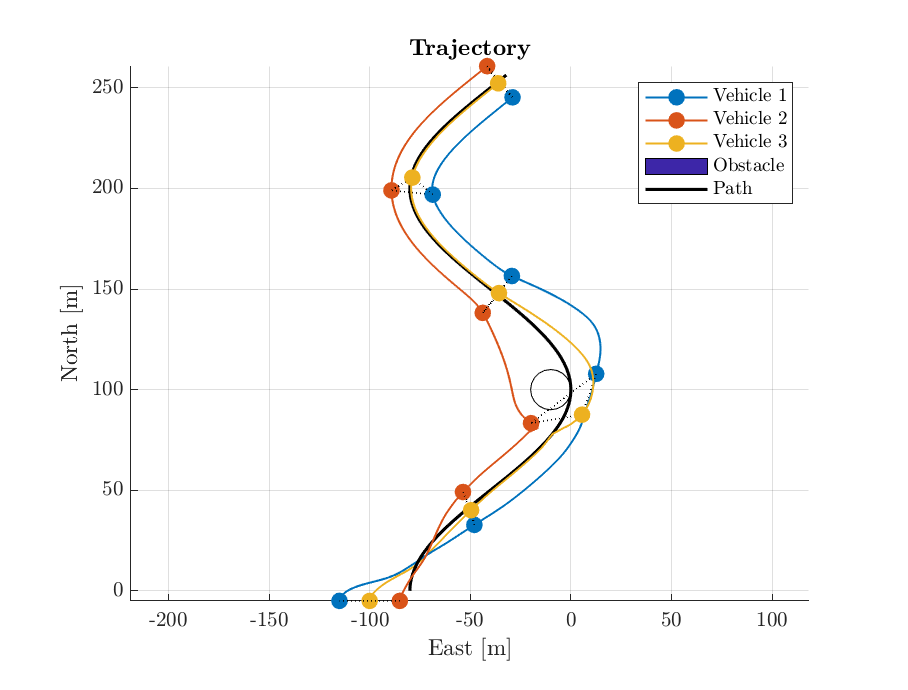
\includegraphics[width=.8\textwidth]{figures/plot3d_IC.eps}
    \vspace*{-4mm}
    \caption{The trajectory of the vehicles. The markers represent the vehicle positions every 50 seconds.}
    \label{fig:plot3d-IC}
    \vspace{-2mm}
\end{figure}

The simulation setup is similar to the previous section, with the same desired path, external obstacle, constant ocean current, and initial states. Furthermore, all controller gains and parameters are also the same, given by Table~\ref{tab:simulation_parameters1}.

The resulting trajectory in the NED coordinate frame is shown in Figure~\ref{fig:plot3d-IC}. The fleet splits up the formation to pass the obstacle and converges back to the formation after the obstacle is passed. Compared to the collision cones avoidance method, the fleet deviates late from the path in order to avoid the obstacle, which is further shown in Figure~\ref{fig:collision_avoidance_IC}, where the green rectangle represents when the external collision avoidance task is active. As also seen in Figure~\ref{fig:collision_avoidance_IC}, the inter-vehicle collision avoidance still works well, despite now being defined as individual tasks for each vehicle, which is expected because the formulation with individual tasks should be equivalent to the joint formulation, as long as only two vehicles are within the collision threshold of each other.

Figure~\ref{fig:path_following_error_IC} shows that the fleet converges earlier to the correct path and deviates minimally from it during the avoidance maneuver. The limited deviation is possible because the path error is defined in terms of the barycenter, and as long as some vehicles of the fleet are on each side of the obstacle, it is possible for the barycenter to remain on the path. Instead, the formation-keeping error increases during the avoidance maneuver, as seen in Figure~\ref{fig:formation_keeping_error_IC}. With the collision cones avoidance method from the previous section, the formation was kept during obstacle avoidance. 

\begin{figure}[htbp]
    \centering
    \begin{subfigure}[t]{.9\textwidth}
    \centering
    \setlength\figurewidth{.8\linewidth}
    \setlength\figureheight{3cm}
    % This file was created by matlab2tikz.
%
%The latest updates can be retrieved from
%  http://www.mathworks.com/matlabcentral/fileexchange/22022-matlab2tikz-matlab2tikz
%where you can also make suggestions and rate matlab2tikz.
%
\definecolor{mycolor1}{rgb}{0.00000,0.44700,0.74100}%
\definecolor{mycolor2}{rgb}{0.85000,0.32500,0.09800}%
%
\begin{tikzpicture}

\begin{axis}[%
width=0.951\figurewidth,
height=\figureheight,
at={(0\figurewidth,0\figureheight)},
scale only axis,
xmin=0,
xmax=250,
xlabel style={at={(axis description cs:0.5,-0.08)}, font=\color{white!15!black}},
xlabel={Time [s]},
ymin=0,
ymax=25,
ylabel style={font=\color{white!15!black}, yshift=2mm},
ylabel={Distance [m]},
axis background/.style={fill=white},
every axis plot/.append style={line width=0.7pt},
title style={font=\bfseries, yshift=-2.75mm},
title={Smallest distances},
legend style={at={(0.97,0.02)}, anchor=south east, legend cell align=left, align=left, draw=white!15!black, legend columns=2,font=\footnotesize}
]
\addplot [color=mycolor1]
  table[]{individual_colav_collision_avoidance-1.tsv};
\addlegendentry{Inter-vehicle}

\addplot [color=mycolor2]
  table[]{individual_colav_collision_avoidance-2.tsv};
\addlegendentry{Obstacle}

\addplot [color=black, dashed]
  table[]{individual_colav_collision_avoidance-3.tsv};
\addlegendentry{$d_{\rm COLAV}$}


\addplot[area legend, dashed, draw=black, fill=white!50!red, fill opacity=0.25, forget plot]
table[] {individual_colav_collision_avoidance-4.tsv}--cycle;

\addplot[area legend, dashed, draw=black, fill=green, fill opacity=0.15, forget plot]
table[] {individual_colav_collision_avoidance-5.tsv}--cycle;
\end{axis}

\end{tikzpicture}%
    \vspace*{-2mm}
    \caption{The minimum inter-vehicle and obstacle distance.}
    \label{fig:collision_avoidance_IC}
    \end{subfigure}
    \\
    \begin{subfigure}[t]{.9\textwidth}
    \centering
    \setlength\figurewidth{.8\linewidth}
    \setlength\figureheight{3.3cm}
    % This file was created by matlab2tikz.
%
%The latest updates can be retrieved from
%  http://www.mathworks.com/matlabcentral/fileexchange/22022-matlab2tikz-matlab2tikz
%where you can also make suggestions and rate matlab2tikz.
%
\definecolor{mycolor1}{rgb}{0.00000,0.44700,0.74100}%
\definecolor{mycolor2}{rgb}{0.85000,0.32500,0.09800}%
\definecolor{mycolor3}{rgb}{0.92900,0.69400,0.12500}%
%
\begin{tikzpicture}

\begin{axis}[%
width=0.951\figurewidth,
height=\figureheight,
at={(0\figurewidth,0\figureheight)},
scale only axis,
xmin=0,
xmax=250,
xlabel style={at={(axis description cs:0.5,-0.08)}, font=\color{white!15!black}},
xlabel={Time [s]},
ymin=-25,
ymax=25,
ylabel style={font=\color{white!15!black}},
ylabel={Error [m]},
axis background/.style={fill=white},
every axis plot/.append style={thick},
title style={font=\bfseries, yshift=-2.75mm},
title={Formation keeping errors},
axis background/.style={fill=white},
legend style={legend cell align=left, align=left, draw=white!15!black,font=\footnotesize}
]
\addplot [color=mycolor1]
  table[]{individual_colav_formation_keeping_error-1.tsv};
  \addlegendentry{$x$-error}
\addplot [color=mycolor1, dashed, forget plot]
  table[]{individual_colav_formation_keeping_error-2.tsv};
\addplot [color=mycolor1, dotted, forget plot]
  table[]{individual_colav_formation_keeping_error-3.tsv};
\addplot [color=mycolor2]
  table[]{individual_colav_formation_keeping_error-4.tsv};
  \addlegendentry{$y$-error}
\addplot [color=mycolor2, dashed, forget plot]
  table[]{individual_colav_formation_keeping_error-5.tsv};
\addplot [color=mycolor2, dotted, forget plot]
  table[]{individual_colav_formation_keeping_error-6.tsv};
\addplot [color=mycolor3]
  table[]{individual_colav_formation_keeping_error-7.tsv};
  \addlegendentry{$z$-error}
\addplot [color=mycolor3, dashed, forget plot]
  table[]{individual_colav_formation_keeping_error-8.tsv};
\addplot [color=mycolor3, dotted, forget plot]
  table[]{individual_colav_formation_keeping_error-9.tsv};

\addplot[area legend, dashed, draw=black, fill=green, fill opacity=0.15, forget plot]
table[] {individual_colav_formation_keeping_error-10.tsv}--cycle;

\addplot[area legend, dashed, draw=black, fill=white!50!red, fill opacity=0.25, forget plot]
table[] {individual_colav_formation_keeping_error-11.tsv}--cycle;
\end{axis}
\end{tikzpicture}%
    \vspace*{-2mm}
    \caption{The formation keeping errors. }
    \label{fig:formation_keeping_error_IC}
    \end{subfigure}
    \\
    \begin{subfigure}[t]{.9\textwidth}
    \centering
    \setlength\figurewidth{.8\linewidth}
    \setlength\figureheight{3cm}
    % This file was created by matlab2tikz.
%
%The latest updates can be retrieved from
%  http://www.mathworks.com/matlabcentral/fileexchange/22022-matlab2tikz-matlab2tikz
%where you can also make suggestions and rate matlab2tikz.
%
\definecolor{mycolor1}{rgb}{0.00000,0.44700,0.74100}%
\definecolor{mycolor2}{rgb}{0.85000,0.32500,0.09800}%
\definecolor{mycolor3}{rgb}{0.92900,0.69400,0.12500}%
%
\begin{tikzpicture}

\begin{axis}[%
width=0.951\figurewidth,
height=\figureheight,
at={(0\figurewidth,0\figureheight)},
scale only axis,
xmin=0,
xmax=250,
xlabel style={at={(axis description cs:0.5,-0.08)}, font=\color{white!15!black}},
xlabel={Time [s]},
ymin=-20,
ymax=5,
ylabel style={font=\color{white!15!black}},
ylabel={Error [m]},
axis background/.style={fill=white},
every axis plot/.append style={line width=0.7pt},
title style={font=\bfseries, yshift=-2.75mm},
title={Path following error},
legend style={legend cell align=left, align=left, draw=white!15!black,font=\footnotesize}
]
\addplot [color=mycolor1]
  table[]{individual_colav_path_following_error-1.tsv};
\addlegendentry{$x$-error}

\addplot [color=mycolor2]
  table[]{individual_colav_path_following_error-2.tsv};
\addlegendentry{$y$-error}

\addplot [color=mycolor3]
  table[]{individual_colav_path_following_error-3.tsv};
\addlegendentry{$z$-error}


\addplot[area legend, dashed, draw=black, fill=green, fill opacity=0.15, forget plot]
table[] {individual_colav_path_following_error-4.tsv}--cycle;
\end{axis}
\end{tikzpicture}%
    \vspace*{-2mm}
    \caption{The path-following error of the barycenter.}
    \label{fig:path_following_error_IC}
    \end{subfigure}
    \vspace*{-2mm}
    \caption{Error variables from the second simulated mission. The full, dashed, and dotted lines correspond to the three different vehicles. The green and red rectangles represent when obstacle avoidance or inter-vehicle COLAV is active.}
    \label{fig:sim_results_IC}
\end{figure}

\begin{figure}[htbp]
    \centering
    \begin{subfigure}[t]{\textwidth}
    \centering
    \setlength\figurewidth{.8\linewidth}
    \setlength\figureheight{4cm}
    % This file was created by matlab2tikz.
%
%The latest updates can be retrieved from
%  http://www.mathworks.com/matlabcentral/fileexchange/22022-matlab2tikz-matlab2tikz
%where you can also make suggestions and rate matlab2tikz.
%
\definecolor{mycolor1}{rgb}{0.00000,0.44700,0.74100}%
\definecolor{mycolor2}{rgb}{0.85000,0.32500,0.09800}%
\definecolor{mycolor3}{rgb}{0.92900,0.69400,0.12500}%
%
\begin{tikzpicture}

\begin{axis}[%
width=0.951\figurewidth,
height=\figureheight,
at={(0\figurewidth,0\figureheight)},
scale only axis,
xmin=0,
xmax=250,
xlabel style={at={(axis description cs:0.5,-0.08)}, font=\color{white!15!black}},
xlabel={Time [s]},
ymin=-0.2,
ymax=0.3,
ylabel style={font=\color{white!15!black}},
ylabel={Angular Velocity [rad/s]},
axis background/.style={fill=white},
title style={font=\bfseries, yshift=-2.75mm},
title={Angular velocities},
axis background/.style={fill=white},
every axis plot/.append style={line width=0.7pt},
legend style={legend cell align=left, align=left, draw=white!15!black, font=\footnotesize}
]
\addplot [color=mycolor1]
  table[]{individual_colav_angular_velocities-1.tsv};
\addlegendentry{Roll rate}

\addplot [color=mycolor1, dashed, forget plot]
  table[]{individual_colav_angular_velocities-2.tsv};
\addplot [color=mycolor1, dotted, forget plot]
  table[]{individual_colav_angular_velocities-3.tsv};
\addplot [color=mycolor2]
  table[]{individual_colav_angular_velocities-4.tsv};
\addlegendentry{Pitch rate}

\addplot [color=mycolor2, dashed, forget plot]
  table[]{individual_colav_angular_velocities-5.tsv};
\addplot [color=mycolor2, dotted, forget plot]
  table[]{individual_colav_angular_velocities-6.tsv};
\addplot [color=mycolor3]
  table[]{individual_colav_angular_velocities-7.tsv};
\addlegendentry{Yaw rate}

\addplot [color=mycolor3, dashed, forget plot]
  table[]{individual_colav_angular_velocities-8.tsv};
\addplot [color=mycolor3, dotted, forget plot]
  table[]{individual_colav_angular_velocities-9.tsv};

\addplot[area legend, dashed, draw=black, fill=green, fill opacity=0.15, forget plot]
table[] {individual_colav_angular_velocities-10.tsv}--cycle;

\addplot[area legend, dashed, draw=black, fill=white!50!red, fill opacity=0.25, forget plot]
table[] {individual_colav_angular_velocities-11.tsv}--cycle;

\end{axis}

\begin{axis}[%
width=1.227\figurewidth,
height=1.227\figureheight,
at={(-0.16\figurewidth,-0.135\figureheight)},
scale only axis,
xmin=0,
xmax=1,
ymin=0,
ymax=1,
axis line style={draw=none},
ticks=none,
axis x line*=bottom,
axis y line*=left
]
\end{axis}
\end{tikzpicture}%
    % \vspace*{-3mm}
    \caption{The angular velocities of the vehicles. Dashed and dotted lines represent different vehicles.}
    \label{fig:angular_velocities_IC}
    \end{subfigure}
    \begin{subfigure}[t]{\textwidth}
    \centering
    \setlength\figurewidth{.8\linewidth}
    \setlength\figureheight{4cm}
    % This file was created by matlab2tikz.
%
%The latest updates can be retrieved from
%  http://www.mathworks.com/matlabcentral/fileexchange/22022-matlab2tikz-matlab2tikz
%where you can also make suggestions and rate matlab2tikz.
%
\definecolor{mycolor1}{rgb}{0.00000,0.44700,0.74100}%
\definecolor{mycolor2}{rgb}{0.85000,0.32500,0.09800}%
\definecolor{mycolor3}{rgb}{0.92900,0.69400,0.12500}%
%
\begin{tikzpicture}

\begin{axis}[%
width=0.951\figurewidth,
height=\figureheight,
at={(0\figurewidth,0\figureheight)},
scale only axis,
xmin=0,
xmax=250,
xlabel style={at={(axis description cs:0.5,-0.08)}, font=\color{white!15!black}},
xlabel={Time [s]},
ymin=0,
ymax=3.5,
ylabel style={font=\color{white!15!black}},
ylabel={Velocity [m/s]},
axis background/.style={fill=white},
every axis plot/.append style={line width=0.7pt},
title style={font=\bfseries, yshift=-2.75mm},
title={Surge velocity},
axis background/.style={fill=white},
legend style={legend pos= north east, legend cell align=left, align=left,  draw=white!15!black, font=\footnotesize}
]
\addplot [color=mycolor1]
  table[]{individual_colav_surge_velocity-1.tsv};
\addlegendentry{First vehicle}
\addplot [color=mycolor2]
  table[]{individual_colav_surge_velocity-2.tsv};
\addlegendentry{Second vehicle}
\addplot [color=mycolor3]
  table[]{individual_colav_surge_velocity-3.tsv};
\addlegendentry{Third vehicle}
  
\addplot [color=black, dashed, forget plot]
  table[]{individual_colav_surge_velocity-4.tsv};

\addplot[area legend, dashed, draw=black, fill=green, fill opacity=0.15, forget plot]
table[] {individual_colav_surge_velocity-5.tsv}--cycle;

\addplot[area legend, dashed, draw=black, fill=white!50!red, fill opacity=0.25, forget plot]
table[] {individual_colav_surge_velocity-6.tsv}--cycle;

\end{axis}
\end{tikzpicture}%
    % \vspace*{-3mm}
    \caption{The surge velocities of the vehicles.}
    \label{fig:surge_velocities_IC}
    \end{subfigure}
    \caption{Angular and surge velocities for the vehicles in the second simulated mission. The green rectangle represents the time when the collision avoidance task was active.}
    \label{fig:velocities_IC}
\end{figure}

Figure~\ref{fig:surge_velocities_IC} shows that the surge velocities of the vehicles rise above $3\, \mathrm{m/s}$ and sink below $0.5\, \mathrm{m/s}$. Velocities above $3\, \mathrm{m/s}$ are unexpected, as it is above the maximum operating velocity of the physical vehicles that the simulation models. There are two possible explanations for such a high velocity. First, the controller might command generalized forces that are larger than the limits of the physical systems actuators. Actuator saturation was not modeled, and such forces would be applied directly to the plant in our simulator. In a real system with actuation limits, the control action going into saturation might impose a stability problem. A second explanation for the large surge velocities is that the simulation does not model non-linear damping. In a more realistic simulator, the non-linear damping would become significant when the velocities increase above the nominal operating range. It is also problematic that the velocity of a vehicle sinks below $0.5\, \mathrm{m/s}$. Then, a real, physical vehicle would lose controllability because water does not flow sufficiently fast past the fins.

\begin{figure}[htb]
    \centering
    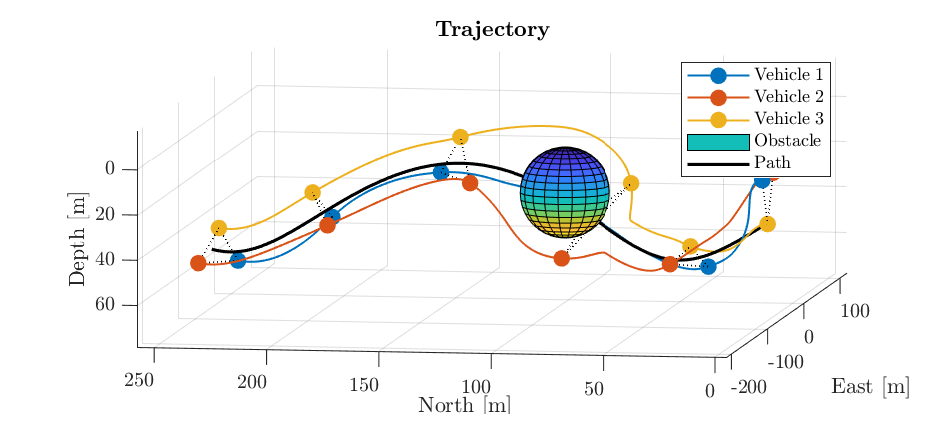
\includegraphics[width=.9\textwidth]{figures/plot3d_sphere.eps}
    \vspace{-3mm}
    \caption{Illustration of obstacle avoidance in all three dimensions. The obstacle is chosen as a sphere.}
    \label{fig:sphere_avoidance}
    \vspace{-4mm}
\end{figure}

Another feature that distinguishes this obstacle avoidance method from the collision cones method is that it enables obstacle avoidance in all three dimensions. In the collision cones method, the avoidance maneuver was limited to the $xy$-plane. As demonstrated in Figure~\ref{fig:sphere_avoidance}, the obstacle avoidance method as described in Section~\ref{sec:individual_colav} enables each individual vehicle to independently avoid the obstacle in all dimensions. The spherical obstacle in this experiment was chosen larger than the cylindrical obstacle in the previous experiments for illustrative purposes.

\subsection{Formation error as damped harmonic motion}\label{sec:harmonic_motion}
Part of the motivation for developing the second-order \gls{nsb} controller is that there are no hidden dynamics abstracted away in the low-level control layer. Consequently, the collision-avoidance and formation-keeping error systems are expected to behave exactly as second-order systems defined by the gain matrices. In turn, the gain matrices can be chosen by specifying natural frequencies and damping ratios as described in Section~\ref{sec:nsb_second_order}. In this section, we will observe the transient of the formation-keeping error under different controller gains. Although we demonstrate the concept with the formation-keeping error, the same behavior is expected for the collision-avoidance task as well.

We design a simple simulation experiment in which everything except for the formation-keeping task is simplified as much as possible. The fleet is made to follow a straight line in the north direction. It is initialized with the barycenter on the path, and there is no external obstacle or ocean current. The desired formation is given by \eqref{eq:desired_formation_sim} as in the previous simulation experiments, and the initial relative positions are given by $\bm{\sigma}_{2,i} = 2\mathbf{p}_{f,i}^f$. All controller gains and parameters except for $k_{p,2}$ and $k_{d,2}$ are given by Table~\ref{tab:simulation_parameters1}. We simulate three different choices of formation-keeping controller gains given by Table~\ref{tab:controller-params}. The natural frequency is kept fixed at $\omega_{n,2} = 0.5$ which is low enough so that the effects of the saturation in the controller are minimal, and the damping ratio is chosen so that the system is underdamped, critically damped, and overdamped for the respective three experiments. The total simulation time is $50\, \mathrm{s}$.

\begin{table}[h]
\centering
\caption{Controller parameters for the three experiments.}
\label{tab:controller-params}
\begin{tabular}{lccc}
\hline
Parameter & Experiment 1 & Experiment 2 & Experiment 3 \\ \hline
$\omega_{n,2}$ & 0.5 & 0.5 & 0.5 \\
$\xi_2$ & 0.3 & 1 & 2 \\
$k_{p,2}$ & 0.25 & 0.25 & 0.25 \\
$k_{d,2}$ & 0.3 & 1 & 2 \\ \hline
\end{tabular}
\end{table}

\begin{figure}[htbp]
    \centering
    \begin{subfigure}[t]{.9\textwidth}
    \centering
    \setlength\figurewidth{.8\linewidth}
    \setlength\figureheight{3.8cm}
    % This file was created by matlab2tikz.
%
%The latest updates can be retrieved from
%  http://www.mathworks.com/matlabcentral/fileexchange/22022-matlab2tikz-matlab2tikz
%where you can also make suggestions and rate matlab2tikz.
%
\definecolor{mycolor1}{rgb}{0.00000,0.44700,0.74100}%
\definecolor{mycolor2}{rgb}{0.85000,0.32500,0.09800}%
\definecolor{mycolor3}{rgb}{0.92900,0.69400,0.12500}%
%
\begin{tikzpicture}

\begin{axis}[%
unit vector ratio*=1 1 1,
width=0.951\figurewidth,
height=\figureheight,
at={(0\figurewidth,0\figureheight)},
scale only axis,
xmin=-50.7157452749055,
xmax=50.7157452749055,
xlabel style={at={(axis description cs:0.5,-0.05)}, font=\color{white!15!black}},
xlabel={East [m]},
ymin=-5,
ymax=74.9999981917057,
ylabel style={font=\color{white!15!black}},
ylabel={North [m]},
axis background/.style={fill=white},
title style={font=\bfseries, yshift=-3mm},
title={\textbf{Trajectory}},
axis x line*=bottom,
axis y line*=left,
xmajorgrids,
ymajorgrids,
legend style={legend cell align=left, align=left, draw=white!15!black, font=\footnotesize}
]
\addplot [color=black, line width=1.5pt]
  table[]{underdamped_3d_plot-4.tsv};
\addlegendentry{Path}

\addplot [color=mycolor1, line width=1.0pt, mark size=3.5pt, mark=*, mark options={solid, fill=mycolor1, mycolor1}, mark repeat = 50]
  table[]{underdamped_3d_plot-1.tsv};
\addlegendentry{Veh. 1}

\addplot [color=mycolor2, line width=1.0pt, mark size=3.5pt, mark=*, mark options={solid, fill=mycolor2, mycolor2}, mark repeat = 50]
  table[]{underdamped_3d_plot-2.tsv};
\addlegendentry{Veh. 2}

\addplot [color=mycolor3, line width=1.0pt, mark size=3.5pt, mark=*, mark options={solid, fill=mycolor3, mycolor3}, mark repeat = 50]
  table[]{underdamped_3d_plot-3.tsv};
\addlegendentry{Veh. 3}



\addplot [color=black, dotted, line width=0.8pt, forget plot]
  table[]{underdamped_3d_plot-5.tsv};
\addplot [color=black, dotted, line width=0.8pt, forget plot]
  table[]{underdamped_3d_plot-6.tsv};
\addplot [color=black, dotted, line width=0.8pt, forget plot]
  table[]{underdamped_3d_plot-7.tsv};
\addplot [color=black, dotted, line width=0.8pt, forget plot]
  table[]{underdamped_3d_plot-8.tsv};
\addplot [color=black, dotted, line width=0.8pt, forget plot]
  table[]{underdamped_3d_plot-9.tsv};
\addplot [color=black, dotted, line width=0.8pt, forget plot]
  table[]{underdamped_3d_plot-10.tsv};
\addplot [color=black, dotted, line width=0.8pt, forget plot]
  table[]{underdamped_3d_plot-11.tsv};
\addplot [color=black, dotted, line width=0.8pt, forget plot]
  table[]{underdamped_3d_plot-12.tsv};
\addplot [color=black, dotted, line width=0.8pt, forget plot]
  table[]{underdamped_3d_plot-13.tsv};
\addplot [color=black, dotted, line width=0.8pt, forget plot]
  table[]{underdamped_3d_plot-14.tsv};
\end{axis}

\end{tikzpicture}%
    \vspace*{-4mm}
    \caption{The underdamped system.}
    \label{fig:underdamped_3d}
    \end{subfigure}
    \vspace*{-.9mm}
    \\
    \begin{subfigure}[t]{.9\textwidth}
    \centering
    \setlength\figurewidth{.8\linewidth}
    \setlength\figureheight{3.8cm}
    % This file was created by matlab2tikz.
%
%The latest updates can be retrieved from
%  http://www.mathworks.com/matlabcentral/fileexchange/22022-matlab2tikz-matlab2tikz
%where you can also make suggestions and rate matlab2tikz.
%
\definecolor{mycolor1}{rgb}{0.00000,0.44700,0.74100}%
\definecolor{mycolor2}{rgb}{0.85000,0.32500,0.09800}%
\definecolor{mycolor3}{rgb}{0.92900,0.69400,0.12500}%
%
\begin{tikzpicture}

\begin{axis}[%
unit vector ratio*=1 1 1,
width=0.951\figurewidth,
height=\figureheight,
at={(0\figurewidth,0\figureheight)},
scale only axis,
xmin=-50.7157485047623,
xmax=50.7157485047623,
xlabel style={at={(axis description cs:0.5,-0.05)}, font=\color{white!15!black}},
xlabel={East [m]},
ymin=-5,
ymax=75.0000032865444,
ylabel style={font=\color{white!15!black}},
ylabel={North [m]},
axis background/.style={fill=white},
title style={font=\bfseries, yshift=-3mm},
title={\textbf{Trajectory}},
axis x line*=bottom,
axis y line*=left,
xmajorgrids,
ymajorgrids,
legend style={legend cell align=left, align=left, draw=white!15!black, font=\footnotesize}
]

\addplot [color=black, line width=1.5pt]
  table[]{critically_damped_3d_plot-4.tsv};
\addlegendentry{Path}

\addplot [color=mycolor1, line width=1.0pt, mark size=3.5pt, mark=*, mark options={solid, fill=mycolor1, mycolor1}, mark repeat=50]
  table[]{critically_damped_3d_plot-1.tsv};
\addlegendentry{Veh. 1}

\addplot [color=mycolor2, line width=1.0pt, mark size=3.5pt, mark=*, mark options={solid, fill=mycolor2, mycolor2}, mark repeat=50]
  table[]{critically_damped_3d_plot-2.tsv};
\addlegendentry{Veh. 2}

\addplot [color=mycolor3, line width=1.0pt, mark size=3.5pt, mark=*, mark options={solid, fill=mycolor3, mycolor3}, mark repeat=50]
  table[]{critically_damped_3d_plot-3.tsv};
\addlegendentry{Veh. 3}



\addplot [color=black, dotted, line width=0.8pt, forget plot]
  table[]{critically_damped_3d_plot-5.tsv};
\addplot [color=black, dotted, line width=0.8pt, forget plot]
  table[]{critically_damped_3d_plot-6.tsv};
\addplot [color=black, dotted, line width=0.8pt, forget plot]
  table[]{critically_damped_3d_plot-7.tsv};
\addplot [color=black, dotted, line width=0.8pt, forget plot]
  table[]{critically_damped_3d_plot-8.tsv};
\addplot [color=black, dotted, line width=0.8pt, forget plot]
  table[]{critically_damped_3d_plot-9.tsv};
\addplot [color=black, dotted, line width=0.8pt, forget plot]
  table[]{critically_damped_3d_plot-10.tsv};
\addplot [color=black, dotted, line width=0.8pt, forget plot]
  table[]{critically_damped_3d_plot-11.tsv};
\addplot [color=black, dotted, line width=0.8pt, forget plot]
  table[]{critically_damped_3d_plot-12.tsv};
\addplot [color=black, dotted, line width=0.8pt, forget plot]
  table[]{critically_damped_3d_plot-13.tsv};
\addplot [color=black, dotted, line width=0.8pt, forget plot]
  table[]{critically_damped_3d_plot-14.tsv};
\end{axis}
\end{tikzpicture}%
    \vspace*{-4mm}
    \caption{The critically damped system. }
    \label{fig:critically_damped_3d}
    \end{subfigure}
    \vspace*{-.9mm}
    \\
    \begin{subfigure}[t]{.9\textwidth}
    \centering
    \setlength\figurewidth{.8\linewidth}
    \setlength\figureheight{3.8cm}
    % This file was created by matlab2tikz.
%
%The latest updates can be retrieved from
%  http://www.mathworks.com/matlabcentral/fileexchange/22022-matlab2tikz-matlab2tikz
%where you can also make suggestions and rate matlab2tikz.
%
\definecolor{mycolor1}{rgb}{0.00000,0.44700,0.74100}%
\definecolor{mycolor2}{rgb}{0.85000,0.32500,0.09800}%
\definecolor{mycolor3}{rgb}{0.92900,0.69400,0.12500}%
%
\begin{tikzpicture}

\begin{axis}[%
unit vector ratio*=1 1 1,
width=0.951\figurewidth,
height=\figureheight,
at={(0\figurewidth,0\figureheight)},
scale only axis,
xmin=-50.7158619100192,
xmax=50.7158619100192,
xlabel style={at={(axis description cs:0.5,-0.05)}, font=\color{white!15!black}},
xlabel={East [m]},
ymin=-5,
ymax=75.0001821741917,
ylabel style={font=\color{white!15!black}},
ylabel={North [m]},
axis background/.style={fill=white},
title style={font=\bfseries, yshift=-3mm},
title={\textbf{Trajectory}},
axis x line*=bottom,
axis y line*=left,
xmajorgrids,
ymajorgrids,
legend style={legend cell align=left, align=left, draw=white!15!black, font=\footnotesize}
]

\addplot [color=black, line width=1.5pt]
  table[]{overdamped_3d_plot-4.tsv};
\addlegendentry{Path}


\addplot [color=mycolor1, line width=1.0pt, mark size=3.5pt, mark=*, mark options={solid, fill=mycolor1, mycolor1}, mark repeat=50]
  table[]{overdamped_3d_plot-1.tsv};
\addlegendentry{Veh. 1}

\addplot [color=mycolor2, line width=1.0pt, mark size=3.5pt, mark=*, mark options={solid, fill=mycolor2, mycolor2}, mark repeat=50]
  table[]{overdamped_3d_plot-2.tsv};
\addlegendentry{Veh. 2}

\addplot [color=mycolor3, line width=1.0pt, mark size=3.5pt, mark=*, mark options={solid, fill=mycolor3, mycolor3}, mark repeat=50]
  table[]{overdamped_3d_plot-3.tsv};
\addlegendentry{Veh. 3}



\addplot [color=black, dotted, line width=0.8pt, forget plot]
  table[]{overdamped_3d_plot-5.tsv};
\addplot [color=black, dotted, line width=0.8pt, forget plot]
  table[]{overdamped_3d_plot-6.tsv};
\addplot [color=black, dotted, line width=0.8pt, forget plot]
  table[]{overdamped_3d_plot-7.tsv};
\addplot [color=black, dotted, line width=0.8pt, forget plot]
  table[]{overdamped_3d_plot-8.tsv};
\addplot [color=black, dotted, line width=0.8pt, forget plot]
  table[]{overdamped_3d_plot-9.tsv};
\addplot [color=black, dotted, line width=0.8pt, forget plot]
  table[]{overdamped_3d_plot-10.tsv};
\addplot [color=black, dotted, line width=0.8pt, forget plot]
  table[]{overdamped_3d_plot-11.tsv};
\addplot [color=black, dotted, line width=0.8pt, forget plot]
  table[]{overdamped_3d_plot-12.tsv};
\addplot [color=black, dotted, line width=0.8pt, forget plot]
  table[]{overdamped_3d_plot-13.tsv};
\addplot [color=black, dotted, line width=0.8pt, forget plot]
  table[]{overdamped_3d_plot-14.tsv};
\end{axis}
\end{tikzpicture}%
    \vspace*{-4mm}
    \caption{The overdamped system.}
    \label{fig:overdamped_3d}
    \end{subfigure}
    \vspace*{-3.5mm}
    \caption{The north-east trajectories of the vehicles with different formation-keeping controller gains.}
    \label{fig:formation_3d_dampings}
\end{figure}


\begin{figure}[htbp]
    \centering
    \begin{subfigure}[t]{.9\textwidth}
    \centering
    \setlength\figurewidth{.8\linewidth}
    \setlength\figureheight{3cm}
    % This file was created by matlab2tikz.
%
%The latest updates can be retrieved from
%  http://www.mathworks.com/matlabcentral/fileexchange/22022-matlab2tikz-matlab2tikz
%where you can also make suggestions and rate matlab2tikz.
%
\definecolor{mycolor1}{rgb}{0.00000,0.44700,0.74100}%
\definecolor{mycolor2}{rgb}{0.85000,0.32500,0.09800}%
\definecolor{mycolor3}{rgb}{0.92900,0.69400,0.12500}%
%
\begin{tikzpicture}

\begin{axis}[%
width=0.951\figurewidth,
height=\figureheight,
at={(0\figurewidth,0\figureheight)},
scale only axis,
xmin=0,
xmax=50,
xlabel style={at={(axis description cs:0.5,-0.08)}, font=\color{white!15!black}},
xlabel={Time [s]},
ymin=-10,
ymax=10,
ylabel style={font=\color{white!15!black}},
ylabel={Error [m]},
axis background/.style={fill=white},
every axis plot/.append style={line width=0.7pt},
title style={font=\bfseries, yshift=-2mm},
title={Formation keeping error},
axis x line*=bottom,
axis y line*=left,
legend style={legend cell align=left, align=left, draw=white!15!black}
]
\addplot [color=mycolor1]
  table[]{underdamped_formation_error-1.tsv};
\addlegendentry{$x$-error}

\addplot [color=mycolor1, dashed, forget plot]
  table[]{underdamped_formation_error-2.tsv};
\addplot [color=mycolor1, dotted, forget plot]
  table[]{underdamped_formation_error-3.tsv};
\addplot [color=mycolor2]
  table[]{underdamped_formation_error-4.tsv};
\addlegendentry{$y$-error}

\addplot [color=mycolor2, dashed, forget plot]
  table[]{underdamped_formation_error-5.tsv};
\addplot [color=mycolor2, dotted, forget plot]
  table[]{underdamped_formation_error-6.tsv};
\addplot [color=mycolor3]
  table[]{underdamped_formation_error-7.tsv};
\addlegendentry{$z$-error}

\addplot [color=mycolor3, dashed, forget plot]
  table[]{underdamped_formation_error-8.tsv};
\addplot [color=mycolor3, dotted, forget plot]
  table[]{underdamped_formation_error-9.tsv};
\end{axis}
\end{tikzpicture}%
    \vspace*{-2mm}
    \caption{The underdamped system.}
    \label{fig:underdamped_formation}
    \end{subfigure}
    \\
    \begin{subfigure}[t]{.9\textwidth}
    \centering
    \setlength\figurewidth{.8\linewidth}
    \setlength\figureheight{3cm}
    % This file was created by matlab2tikz.
%
%The latest updates can be retrieved from
%  http://www.mathworks.com/matlabcentral/fileexchange/22022-matlab2tikz-matlab2tikz
%where you can also make suggestions and rate matlab2tikz.
%
\definecolor{mycolor1}{rgb}{0.00000,0.44700,0.74100}%
\definecolor{mycolor2}{rgb}{0.85000,0.32500,0.09800}%
\definecolor{mycolor3}{rgb}{0.92900,0.69400,0.12500}%
%
\begin{tikzpicture}

\begin{axis}[%
width=0.951\figurewidth,
height=\figureheight,
at={(0\figurewidth,0\figureheight)},
scale only axis,
xmin=0,
xmax=50,
xlabel style={at={(axis description cs:0.5,-0.08)},font=\color{white!15!black}},
xlabel={Time [s]},
ymin=-10,
ymax=10,
ylabel style={ font=\color{white!15!black}},
ylabel={Error [m]},
axis background/.style={fill=white},
every axis plot/.append style={line width=0.7pt},
title style={font=\bfseries, yshift=-2mm},
title={Formation keeping error},
axis x line*=bottom,
axis y line*=left,
legend style={legend cell align=left, align=left, draw=white!15!black}
]
\addplot [color=mycolor1]
  table[]{critically_damped_formation_error-1.tsv};
\addlegendentry{$x$-error}

\addplot [color=mycolor1, dashed, forget plot]
  table[]{critically_damped_formation_error-2.tsv};
\addplot [color=mycolor1, dotted, forget plot]
  table[]{critically_damped_formation_error-3.tsv};
\addplot [color=mycolor2]
  table[]{critically_damped_formation_error-4.tsv};
\addlegendentry{$y$-error}

\addplot [color=mycolor2, dashed, forget plot]
  table[]{critically_damped_formation_error-5.tsv};
\addplot [color=mycolor2, dotted, forget plot]
  table[]{critically_damped_formation_error-6.tsv};
\addplot [color=mycolor3]
  table[]{critically_damped_formation_error-7.tsv};
\addlegendentry{$z$-error}

\addplot [color=mycolor3, dashed, forget plot]
  table[]{critically_damped_formation_error-8.tsv};
\addplot [color=mycolor3, dotted, forget plot]
  table[]{critically_damped_formation_error-9.tsv};
\end{axis}

\end{tikzpicture}%
    \vspace*{-2mm}
    \caption{The critically damped system. }
    \label{fig:critically_damped_formation}
    \end{subfigure}
    \\
    \begin{subfigure}[t]{.9\textwidth}
    \centering
    \setlength\figurewidth{.8\linewidth}
    \setlength\figureheight{3cm}
    % This file was created by matlab2tikz.
%
%The latest updates can be retrieved from
%  http://www.mathworks.com/matlabcentral/fileexchange/22022-matlab2tikz-matlab2tikz
%where you can also make suggestions and rate matlab2tikz.
%
\definecolor{mycolor1}{rgb}{0.00000,0.44700,0.74100}%
\definecolor{mycolor2}{rgb}{0.85000,0.32500,0.09800}%
\definecolor{mycolor3}{rgb}{0.92900,0.69400,0.12500}%
%
\begin{tikzpicture}

\begin{axis}[%
width=0.951\figurewidth,
height=\figureheight,
at={(0\figurewidth,0\figureheight)},
scale only axis,
xmin=0,
xmax=50,
xlabel style={at={(axis description cs:0.5,-0.08)}, font=\color{white!15!black}},
xlabel={Time [s]},
ymin=-10,
ymax=10,
ylabel style={font=\color{white!15!black}},
ylabel={Error [m]},
axis background/.style={fill=white},
every axis plot/.append style={line width=0.7pt},
title style={font=\bfseries, yshift=-2mm},
title={Formation keeping error},
axis x line*=bottom,
axis y line*=left,
legend style={legend cell align=left, align=left, draw=white!15!black}
]
\addplot [color=mycolor1]
  table[]{overdamped_formation_error-1.tsv};
\addlegendentry{$x$-error}

\addplot [color=mycolor1, dashed, forget plot]
  table[]{overdamped_formation_error-2.tsv};
\addplot [color=mycolor1, dotted, forget plot]
  table[]{overdamped_formation_error-3.tsv};
\addplot [color=mycolor2]
  table[]{overdamped_formation_error-4.tsv};
\addlegendentry{$y$-error}

\addplot [color=mycolor2, dashed, forget plot]
  table[]{overdamped_formation_error-5.tsv};
\addplot [color=mycolor2, dotted, forget plot]
  table[]{overdamped_formation_error-6.tsv};
\addplot [color=mycolor3]
  table[]{overdamped_formation_error-7.tsv};
\addlegendentry{$z$-error}

\addplot [color=mycolor3, dashed, forget plot]
  table[]{overdamped_formation_error-8.tsv};
\addplot [color=mycolor3, dotted, forget plot]
  table[]{overdamped_formation_error-9.tsv};
\end{axis}
\end{tikzpicture}%
    \vspace*{-2mm}
    \caption{The overdamped system.}
    \label{fig:overdamped_formation}
    \end{subfigure}
    \vspace*{-2mm}
    \caption{The formation-keeping errors for the vehicles with different formation-keeping controller gains. The full, dashed, and dotted lines illustrate the different vehicles.}
    \label{fig:formation_dampings_errors}
\end{figure}

Figure~\ref{fig:formation_3d_dampings} shows the north-east trajectory for the vehicles with different damping ratios. The corresponding formation-keeping errors are shown in Figure~\ref{fig:formation_dampings_errors}. As expected, the formation-keeping error in the underdamped system exhibits an oscillatory motion. The error in the critically damped system converges quickly to the origin without oscillations, and the overdamped system converges more slowly. Despite the saturation term in the formation-keeping acceleration \eqref{eq:saturated_formation_keeping}, the task errors converge as can be expected from the theory of damped harmonic motion.

\vspace{-3mm}
\section{Distributed NSB algorithm simulation results}\label{sec:distributed_simulations}
This section presents three simulation experiments with the distributed \gls{nsb} method from Chapter~\ref{cha:distributed_NSB}. The method is first demonstrated on a general mission featuring collision avoidance, formation keeping, and path following in Section~\ref{sec:simulation_distributed_nsb}. Then, the method is compared to two existing methods from the literature in Sections~\ref{sec:comparison_distributed_NSB} and \ref{sec:comparison_restrepo}, and the alternative distributed implementation in Section~\ref{sec:sim_alternative}. The method is configured with the sliding-mode path-following acceleration given by \eqref{eq:sliding_mode_path_following}.


\subsection{General five-agent mission}\label{sec:simulation_distributed_nsb}
This section presents a simulation experiment of the distributed \gls{nsb} control law presented in Chapter~\ref{cha:distributed_NSB}. The experiment involves a fleet of five agents with a communication graph given by Figure~\ref{fig:communication_graph}. All controller gains and parameters are unchanged from previous experiments and given by Table~\ref{tab:simulation_parameters1}.
\begin{figure}[h]
    \centering
    \begin{tikzpicture}
  % Nodes
  \node[circle, draw, minimum size=6mm] (1) at (0,0) {1};
  \node[circle, draw, minimum size=6mm] (2) at (-2,0) {2};
  \node[circle, draw, minimum size=6mm] (3) at (-1,{sqrt(2)}) {3};
  \node[circle, draw, minimum size=6mm] (4) at (2,0) {4};
  \node[circle, draw, minimum size=6mm] (5) at (1,{sqrt(2)}) {5};
  
  % Edges
  \foreach \x/\y/\name in {1/2/$e_1$, 2/3/$e_2$, 3/1/$e_3$, 4/1/$e_4$, 5/4/$e_5$, 1/5/$e_6$}
    \draw (\x) -- (\y) node[midway, auto] {\name};
\end{tikzpicture}
\vspace*{-4mm}
    \caption{The communication graph of the fleet.}
    \label{fig:communication_graph}
    \vspace*{-4mm}
\end{figure}


The barycenter relative vectors give the desired formation:
\begin{equation}
    \begin{split}
    \mathbf{p}_{f,1:5}^f = \begin{bmatrix}
        0 & 8 & 8 & -8 & -8\\ 0 & -8 & 8 & 8 & -8 \\ 8 & -2& -2& -2& -2
    \end{bmatrix}.
    % ,\; \mathbf{p}_{f,2}^f = &\begin{bmatrix}
    %     8 \\ -8 \\ -2
    % \end{bmatrix},\; \mathbf{p}_{f,3}^f = \begin{bmatrix}
    %     8 \\ 8 \\ -2
    % \end{bmatrix},\; \\
    % \mathbf{p}_{f,4}^f = \begin{bmatrix}
    %     -8 \\ 8 \\ -2
    % \end{bmatrix}&,\; \mathbf{p}_{f,5}^f = \begin{bmatrix}
    %     -8 \\ -8 \\ -2
    % \end{bmatrix}.
    \end{split}
\end{equation}
The desired formation-relative positions of the agents 2-5 make up a square in the $xy$-plane. The fleet is initialized so that each of the four agents starts at opposite corners of the square. The initial positions are chosen slightly closer than the desired formation so that the inter-vehicle collision avoidance task activates:
\begin{equation}
    \begin{split}
    \mathbf{p}_{1:5}(0) = \begin{bmatrix}
        0 &-5& -5& 5& 5\\ 0 & 5 & -5 & -5 & 5\\ 5 & -1.25& -1.25& -1.25& -1.25
    \end{bmatrix}.
    % ,\; \mathbf{p}_{2}(0) = &\begin{bmatrix}
    %     -5 \\ 5 \\ -1.25
    % \end{bmatrix},\; \mathbf{p}_{3}(0) = \begin{bmatrix}
    %     -5 \\ -5 \\ -1.25
    % \end{bmatrix},\; \\
    % \mathbf{p}_{4}(0) = \begin{bmatrix}
    %     5 \\ -5 \\ -1.25
    % \end{bmatrix}&,\; \mathbf{p}_{5}(0) = \begin{bmatrix}
    %     5 \\ 5 \\ -1.25
    % \end{bmatrix}.
    \end{split}
\end{equation}

The fleet avoids the obstacle and converges to the desired path as seen by Figure~\ref{fig:distributed_path_plot}. Figure~\ref{fig:distributed_sim_results} shows more clearly that the formation-keeping and path-following errors converge to and remain at zero. Figure~\ref{fig:distributed_collision_avoidance} shows that the collision avoidance task works similarly to the centralized algorithm, with only small violations of the collision-avoidance threshold. 
\begin{figure}[hb]
    \centering
    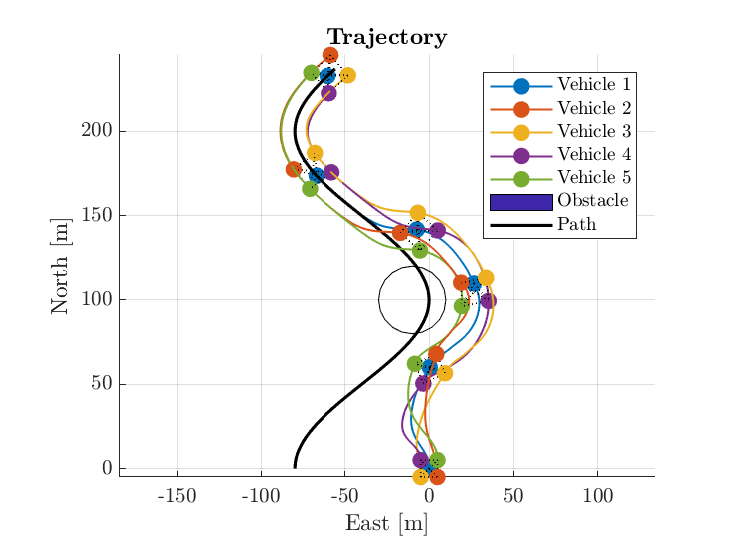
\includegraphics[width=.8\textwidth]{figures/distributed_path_plot.eps}
    \vspace{-4mm}
    \caption{The trajectory of the fleet in the North-East frame.}
    \label{fig:distributed_path_plot}
    \vspace{-4mm}
\end{figure}

\begin{figure}[htbp]
    \centering
    \begin{subfigure}[t]{.9\textwidth}
    \centering
    \setlength\figurewidth{.8\linewidth}
    \setlength\figureheight{3cm}
    % This file was created by matlab2tikz.
%
%The latest updates can be retrieved from
%  http://www.mathworks.com/matlabcentral/fileexchange/22022-matlab2tikz-matlab2tikz
%where you can also make suggestions and rate matlab2tikz.
%
\definecolor{mycolor1}{rgb}{0.00000,0.44700,0.74100}%
\definecolor{mycolor2}{rgb}{0.85000,0.32500,0.09800}%
%
\begin{tikzpicture}

\begin{axis}[%
width=0.951\figurewidth,
height=\figureheight,
at={(0\figurewidth,0\figureheight)},
scale only axis,
xmin=0,
xmax=250,
xlabel style={font=\color{white!15!black}},
xlabel={Time [s]},
ymin=0,
ymax=20,
ylabel style={font=\color{white!15!black}, yshift=2mm},
ylabel={Distance [m]},
axis background/.style={fill=white},
every axis plot/.append style={line width=0.7pt},
title style={font=\bfseries, yshift=-2.75mm},
title={Smallest distances},
legend style={at={(0.97,0.02)}, anchor=south east, legend cell align=left, align=left, draw=white!15!black, legend columns=2,font=\footnotesize}
]
\addplot [color=mycolor1]
  table[]{distributed_colav-1.tsv};
\addlegendentry{Inter-vehicle distance}

\addplot [color=mycolor2]
  table[]{distributed_colav-2.tsv};
\addlegendentry{Distance to obstacle}

\addplot [color=black, dashed]
  table[]{distributed_colav-3.tsv};
\addlegendentry{$d_{\rm COLAV}$}


\addplot[area legend, dashed, draw=black, fill=white!50!red, fill opacity=0.25, forget plot]
table[] {distributed_colav-4.tsv}--cycle;

\addplot[area legend, dashed, draw=black, fill=green, fill opacity=0.15, forget plot]
table[] {distributed_colav-5.tsv}--cycle;
\end{axis}

\begin{axis}[%
width=1.227\figurewidth,
height=1.227\figureheight,
at={(-0.16\figurewidth,-0.135\figureheight)},
scale only axis,
xmin=0,
xmax=1,
ymin=0,
ymax=1,
axis line style={draw=none},
ticks=none,
axis x line*=bottom,
axis y line*=left
]
\end{axis}
\end{tikzpicture}%
    \vspace*{-2mm}
    \caption{The minimum inter-vehicle and obstacle distance.}
    \label{fig:distributed_collision_avoidance}
    \end{subfigure}
    \\
    \begin{subfigure}[t]{.9\textwidth}
    \centering
    \setlength\figurewidth{.8\linewidth}
    \setlength\figureheight{3cm}
    % This file was created by matlab2tikz.
%
%The latest updates can be retrieved from
%  http://www.mathworks.com/matlabcentral/fileexchange/22022-matlab2tikz-matlab2tikz
%where you can also make suggestions and rate matlab2tikz.
%
\definecolor{mycolor1}{rgb}{0.00000,0.44700,0.74100}%
\definecolor{mycolor2}{rgb}{0.85000,0.32500,0.09800}%
\definecolor{mycolor3}{rgb}{0.92900,0.69400,0.12500}%
%
\begin{tikzpicture}

\begin{axis}[%
width=0.951\figurewidth,
height=\figureheight,
at={(0\figurewidth,0\figureheight)},
scale only axis,
xmin=0,
xmax=250,
xlabel style={font=\color{white!15!black}},
xlabel={Time [s]},
ymin=-15,
ymax=15,
ylabel style={font=\color{white!15!black}},
ylabel={Error [m]},
axis background/.style={fill=white},
title style={font=\bfseries, yshift=-2.75mm},
title={Formation keeping errors},
axis background/.style={fill=white},
every axis plot/.append style={line width=0.7pt},
legend style={legend cell align=left, align=left, draw=white!15!black,font=\footnotesize}
]
\addplot [color=mycolor1]
  table[]{distributed_formation_keeping-1.tsv};
  \addlegendentry{$x$-error}
\addplot [color=mycolor1, dashed, forget plot]
  table[]{distributed_formation_keeping-2.tsv};
\addplot [color=mycolor1, dotted, forget plot]
  table[]{distributed_formation_keeping-3.tsv};
\addplot [color=mycolor1, dashdotted, forget plot]
  table[]{distributed_formation_keeping-4.tsv};
\addplot [color=mycolor1, forget plot]
  table[]{distributed_formation_keeping-5.tsv};
\addplot [color=mycolor2]
  table[]{distributed_formation_keeping-6.tsv};
\addlegendentry{$y$-error}
\addplot [color=mycolor2, dashed, forget plot]
  table[]{distributed_formation_keeping-7.tsv};
\addplot [color=mycolor2, dotted, forget plot]
  table[]{distributed_formation_keeping-8.tsv};
\addplot [color=mycolor2, dashdotted, forget plot]
  table[]{distributed_formation_keeping-9.tsv};
\addplot [color=mycolor2, forget plot]
  table[]{distributed_formation_keeping-10.tsv};
\addplot [color=mycolor3]
  table[]{distributed_formation_keeping-11.tsv};
  \addlegendentry{$z$-error}
\addplot [color=mycolor3, dashed, forget plot]
  table[]{distributed_formation_keeping-12.tsv};
\addplot [color=mycolor3, dotted, forget plot]
  table[]{distributed_formation_keeping-13.tsv};
\addplot [color=mycolor3, dashdotted, forget plot]
  table[]{distributed_formation_keeping-14.tsv};
\addplot [color=mycolor3, forget plot]
  table[]{distributed_formation_keeping-15.tsv};

\addplot[area legend, dashed, draw=black, fill=green, fill opacity=0.15, forget plot]
table[] {distributed_formation_keeping-16.tsv}--cycle;

\addplot[area legend, dashed, draw=black, fill=white!50!red, fill opacity=0.25, forget plot]
table[] {distributed_formation_keeping-17.tsv}--cycle;
\end{axis}

\begin{axis}[%
width=1.227\figurewidth,
height=1.227\figureheight,
at={(-0.16\figurewidth,-0.135\figureheight)},
scale only axis,
xmin=0,
xmax=1,
ymin=0,
ymax=1,
axis line style={draw=none},
ticks=none,
axis x line*=bottom,
axis y line*=left
]
\end{axis}
\end{tikzpicture}%
    \vspace*{-2mm}
    \caption{The formation keeping errors. }
    \label{fig:distributed_formation_keeping_error}
    \end{subfigure}
    \\
    \begin{subfigure}[t]{.9\textwidth}
    \centering
    \setlength\figurewidth{.8\linewidth}
    \setlength\figureheight{3cm}
    % This file was created by matlab2tikz.
%
%The latest updates can be retrieved from
%  http://www.mathworks.com/matlabcentral/fileexchange/22022-matlab2tikz-matlab2tikz
%where you can also make suggestions and rate matlab2tikz.
%
\definecolor{mycolor1}{rgb}{0.00000,0.44700,0.74100}%
\definecolor{mycolor2}{rgb}{0.85000,0.32500,0.09800}%
\definecolor{mycolor3}{rgb}{0.92900,0.69400,0.12500}%
%
\begin{tikzpicture}

\begin{axis}[%
width=0.951\figurewidth,
height=\figureheight,
at={(0\figurewidth,0\figureheight)},
scale only axis,
xmin=0,
xmax=250,
xlabel style={font=\color{white!15!black}},
xlabel={Time [s]},
ymin=-60,
ymax=80,
ylabel style={font=\color{white!15!black}},
ylabel={Error [m]},
axis background/.style={fill=white},
every axis plot/.append style={line width=0.7pt},
title style={font=\bfseries, yshift=-2.75mm},
title={Path following error},
legend style={legend cell align=left, align=left, draw=white!15!black,font=\footnotesize}
]
\addplot [color=mycolor1]
  table[]{distributed_path_following-1.tsv};
\addlegendentry{$x$-error}

\addplot [color=mycolor2]
  table[]{distributed_path_following-2.tsv};
\addlegendentry{$y$-error}

\addplot [color=mycolor3]
  table[]{distributed_path_following-3.tsv};
\addlegendentry{$z$-error}


\addplot[area legend, dashed, draw=black, fill=green, fill opacity=0.15, forget plot]
table[] {distributed_path_following-4.tsv}--cycle;
\end{axis}
\end{tikzpicture}%
    \vspace*{-2mm}
    \caption{The path-following error of the barycenter.}
    \label{fig:distributed_path_following_error}
    \end{subfigure}
    \vspace*{-2mm}
    \caption{Error variables from the simulated distributed mission. The different line styles correspond to the five different vehicles. The green and red rectangles represent when obstacle avoidance or inter-vehicle COLAV is active.}
    \label{fig:distributed_sim_results}
\end{figure}

\subsection{Comparison study with the first-order NSB method}\label{sec:comparison_distributed_NSB}
In this section, we compare our distributed \gls{nsb} method with the first-order \gls{nsb} method from \cite{matous_formation_2023}. The Simulink model for the first-order method was provided by Josef Matou\v{s}. The first-order method is implemented in a  distributed manner as described in Section~\ref{sec:alternative_distributed}. 

We simulate the two methods on the four-vehicle simulation experiment detailed in \cite{matous_formation_2023}. We choose the experiment without obstacles because the two methods implement obstacle avoidance differently. Furthermore, the inter-vehicle collision avoidance threshold is chosen small enough for the task to not activate because the provided implementation of the first-order \gls{nsb} does not include that task. The barycenter should follow an elliptic path given by
\begin{equation}
    \mathbf{p}_p(\xi) = [a \cos{\xi},\, b \sin{\xi},\, c\sin{\xi}^2]\T,
\end{equation}
where $a = 60\, \mathrm{m}$, $b = 40\, \mathrm{m}$, $c = 10\, \mathrm{m}$. The shape of the desired formation is given by 
\begin{equation}
    \mathbf{p}_{f,1:4}^f = \begin{bmatrix}
      10& -10&  0&   0\\
      0&   0& 10& -10\\
      0&  -4&  4&   0
    \end{bmatrix},
\end{equation}
and the communication graph is given by Figure~\ref{fig:communication_graph_comparison}.
\begin{figure}[hb]
    \centering
     \begin{tikzpicture}
  % Nodes
  \node[circle, draw, minimum size=6mm] (1) at (0,0) {1};
  \node[circle, draw, minimum size=6mm] (2) at (3,0) {2};
  \node[circle, draw, minimum size=6mm] (3) at (3,3) {3};
  \node[circle, draw, minimum size=6mm] (4) at (0,3) {4};
  
  % Edges
  \foreach \x/\y/\name in {1/3/$e_1$, 1/4/$e_2$, 2/3/$e_3$, 2/4/$e_4$}
    \draw (\x) -- (\y) node[midway,auto, xshift=-2mm] {\name};
\end{tikzpicture}
    \caption{Communication graph for the comparison experiment.}
    \label{fig:communication_graph_comparison}
\end{figure}

\begin{figure}[ht]
    \centering
    \setlength\figurewidth{.7\textwidth}
    \setlength\figureheight{0.5\textwidth}
    % This file was created by matlab2tikz.
%
%The latest updates can be retrieved from
%  http://www.mathworks.com/matlabcentral/fileexchange/22022-matlab2tikz-matlab2tikz
%where you can also make suggestions and rate matlab2tikz.
%
\definecolor{mycolor1}{rgb}{0.00000,0.44700,0.74100}%
\definecolor{mycolor2}{rgb}{0.85000,0.32500,0.09800}%
\definecolor{mycolor3}{rgb}{0.92900,0.69400,0.12500}%
\definecolor{mycolor4}{rgb}{0.49400,0.18400,0.55600}%
%
\begin{tikzpicture}

\begin{axis}[%
% unit vector ratio*=1 1 1,
width=\figurewidth,
height=0.794\figureheight,
at={(0\figurewidth,0\figureheight)},
scale only axis,
plot box ratio=6.842 5.397 1,
xmin=-95.0778035133361,
xmax=95.1001524564096,
tick align=outside,
xlabel style={font=\color{white!15!black}},
xlabel={East [m]},
ymin=-69.9951943051704,
ymax=80,
ylabel style={font=\color{white!15!black}},
ylabel={North [m]},
z dir=reverse,
zmin=-9.16458892913122,
zmax=18.6292631457881,
zlabel style={font=\color{white!15!black}},
zlabel={Depth [m]},
view={-86.2420632235235}{20},
axis background/.style={fill=white},
title style={font=\bfseries},
title={\textbf{Trajectory}},
axis x line*=bottom,
axis y line*=left,
axis z line*=left,
xmajorgrids,
ymajorgrids,
zmajorgrids,
legend style={legend cell align=left, align=left, draw=white!15!black, legend columns=5,font=\footnotesize}
]
\addplot3 [color=mycolor1, line width=1.0pt, mark size=3.5pt, mark=*, mark options={solid, fill=mycolor1, mycolor1}, mark repeat= 50]
 table[] {path_3d_comparison-1.tsv};
 \addlegendentry{AUV 1}

\addplot3 [color=mycolor2, line width=1.0pt, mark size=3.5pt, mark=*, mark options={solid, fill=mycolor2, mycolor2}, mark repeat= 50]
 table[] {path_3d_comparison-2.tsv};
 \addlegendentry{AUV 2}

\addplot3 [color=mycolor3, line width=1.0pt, mark size=3.5pt, mark=*, mark options={solid, fill=mycolor3, mycolor3}, mark repeat= 50]
 table[] {path_3d_comparison-3.tsv};
 \addlegendentry{AUV 3}

\addplot3 [color=mycolor4, line width=1.0pt, mark size=3.5pt, mark=*, mark options={solid, fill=mycolor4, mycolor4}, mark repeat= 50]
 table[] {path_3d_comparison-4.tsv};
 \addlegendentry{AUV 4}

\addplot3 [color=black, line width=1.5pt]
 table[] {path_3d_comparison-5.tsv};
 \addlegendentry{Path}

\addplot3 [color=black, dotted, line width=0.8pt]
 table[] {path_3d_comparison-6.tsv};
 \addplot3 [color=black, dotted, line width=0.8pt]
 table[] {path_3d_comparison-7.tsv};
 \addplot3 [color=black, dotted, line width=0.8pt]
 table[] {path_3d_comparison-8.tsv};
 \addplot3 [color=black, dotted, line width=0.8pt]
 table[] {path_3d_comparison-9.tsv};
 \addplot3 [color=black, dotted, line width=0.8pt]
 table[] {path_3d_comparison-10.tsv};
 \addplot3 [color=black, dotted, line width=0.8pt]
 table[] {path_3d_comparison-11.tsv};
 \addplot3 [color=black, dotted, line width=0.8pt]
 table[] {path_3d_comparison-12.tsv};
 \addplot3 [color=black, dotted, line width=0.8pt]
 table[] {path_3d_comparison-13.tsv};
 \addplot3 [color=black, dotted, line width=0.8pt]
 table[] {path_3d_comparison-14.tsv};
 \addplot3 [color=black, dotted, line width=0.8pt]
 table[] {path_3d_comparison-15.tsv};
 \addplot3 [color=black, dotted, line width=0.8pt]
 table[] {path_3d_comparison-16.tsv};
 \addplot3 [color=black, dotted, line width=0.8pt]
 table[] {path_3d_comparison-17.tsv};
 \addplot3 [color=black, dotted, line width=0.8pt]
 table[] {path_3d_comparison-18.tsv};
 \addplot3 [color=black, dotted, line width=0.8pt]
 table[] {path_3d_comparison-19.tsv};
 \addplot3 [color=black, dotted, line width=0.8pt]
 table[] {path_3d_comparison-20.tsv};
 \addplot3 [color=black, dotted, line width=0.8pt]
 table[] {path_3d_comparison-21.tsv};
 \addplot3 [color=black, dotted, line width=0.8pt]
 table[] {path_3d_comparison-22.tsv};
 \addplot3 [color=black, dotted, line width=0.8pt]
 table[] {path_3d_comparison-23.tsv};
 \addplot3 [color=black, dotted, line width=0.8pt]
 table[] {path_3d_comparison-24.tsv};
 \addplot3 [color=black, dotted, line width=0.8pt]
 table[] {path_3d_comparison-25.tsv};
 \addplot3 [color=black, dotted, line width=0.8pt]
 table[] {path_3d_comparison-26.tsv};
 \addplot3 [color=black, dotted, line width=0.8pt]
 table[] {path_3d_comparison-27.tsv};
 \addplot3 [color=black, dotted, line width=0.8pt]
 table[] {path_3d_comparison-28.tsv};
 \addplot3 [color=black, dotted, line width=0.8pt]
 table[] {path_3d_comparison-29.tsv};
 \addplot3 [color=black, dotted, line width=0.8pt]
 table[] {path_3d_comparison-30.tsv};
 \addplot3 [color=black, dotted, line width=0.8pt]
 table[] {path_3d_comparison-31.tsv};
 \addplot3 [color=black, dotted, line width=0.8pt]
 table[] {path_3d_comparison-32.tsv};
 \addplot3 [color=black, dotted, line width=0.8pt]
 table[] {path_3d_comparison-33.tsv};
 \addplot3 [color=black, dotted, line width=0.8pt]
 table[] {path_3d_comparison-34.tsv};
 \addplot3 [color=black, dotted, line width=0.8pt]
 table[] {path_3d_comparison-35.tsv};
 \addplot3 [color=black, dotted, line width=0.8pt]
 table[] {path_3d_comparison-36.tsv};
 \addplot3 [color=black, dotted, line width=0.8pt]
 table[] {path_3d_comparison-37.tsv};
 \addplot3 [color=black, dotted, line width=0.8pt]
 table[] {path_3d_comparison-38.tsv};
 \addplot3 [color=black, dotted, line width=0.8pt]
 table[] {path_3d_comparison-39.tsv};
 \addplot3 [color=black, dotted, line width=0.8pt]
 table[] {path_3d_comparison-40.tsv};
 \addplot3 [color=black, dotted, line width=0.8pt]
 table[] {path_3d_comparison-41.tsv};
 \addplot3 [color=black, dotted, line width=0.8pt]
 table[] {path_3d_comparison-42.tsv};
 \addplot3 [color=black, dotted, line width=0.8pt]
 table[] {path_3d_comparison-43.tsv};
 \addplot3 [color=black, dotted, line width=0.8pt]
 table[] {path_3d_comparison-44.tsv};
 \addplot3 [color=black, dotted, line width=0.8pt]
 table[] {path_3d_comparison-45.tsv};
 \addplot3 [color=black, dotted, line width=0.8pt]
 table[] {path_3d_comparison-46.tsv};
 \addplot3 [color=black, dotted, line width=0.8pt]
 table[] {path_3d_comparison-47.tsv};
 \addplot3 [color=black, dotted, line width=0.8pt]
 table[] {path_3d_comparison-48.tsv};
 \addplot3 [color=black, dotted, line width=0.8pt]
 table[] {path_3d_comparison-49.tsv};
 \addplot3 [color=black, dotted, line width=0.8pt]
 table[] {path_3d_comparison-50.tsv};
 \addplot3 [color=black, dotted, line width=0.8pt]
 table[] {path_3d_comparison-51.tsv};
 \addplot3 [color=black, dotted, line width=0.8pt]
 table[] {path_3d_comparison-52.tsv};
 \addplot3 [color=black, dotted, line width=0.8pt]
 table[] {path_3d_comparison-53.tsv};
 \addplot3 [color=black, dotted, line width=0.8pt]
 table[] {path_3d_comparison-54.tsv};
 \addplot3 [color=black, dotted, line width=0.8pt]
 table[] {path_3d_comparison-55.tsv};
 \addplot3 [color=black, dotted, line width=0.8pt]
 table[] {path_3d_comparison-56.tsv};
 \addplot3 [color=black, dotted, line width=0.8pt]
 table[] {path_3d_comparison-57.tsv};
 \addplot3 [color=black, dotted, line width=0.8pt]
 table[] {path_3d_comparison-58.tsv};
 \addplot3 [color=black, dotted, line width=0.8pt]
 table[] {path_3d_comparison-59.tsv};
 \addplot3 [color=black, dotted, line width=0.8pt]
 table[] {path_3d_comparison-60.tsv};
 \addplot3 [color=black, dotted, line width=0.8pt]
 table[] {path_3d_comparison-61.tsv};
 \addplot3 [color=black, dotted, line width=0.8pt]
 table[] {path_3d_comparison-62.tsv};
 \addplot3 [color=black, dotted, line width=0.8pt]
 table[] {path_3d_comparison-63.tsv};
 \addplot3 [color=black, dotted, line width=0.8pt]
 table[] {path_3d_comparison-64.tsv};
 \addplot3 [color=black, dotted, line width=0.8pt]
 table[] {path_3d_comparison-65.tsv};
 \addplot3 [color=black, dotted, line width=0.8pt]
 table[] {path_3d_comparison-66.tsv};
 \addplot3 [color=black, dotted, line width=0.8pt]
 table[] {path_3d_comparison-67.tsv};
 \addplot3 [color=black, dotted, line width=0.8pt]
 table[] {path_3d_comparison-68.tsv};
 \end{axis}

\begin{axis}[%
width=1.32\figurewidth,
height=1.32\figureheight,
at={(-0.172\figurewidth,-0.286\figureheight)},
scale only axis,
xmin=0,
xmax=1,
ymin=0,
ymax=1,
axis line style={draw=none},
ticks=none,
axis x line*=bottom,
axis y line*=left
]
\end{axis}
\end{tikzpicture}%
    \vspace*{-4mm}
    \caption{The 3D trajectory from the second-order \gls{nsb} method in the comparison experiment.}
    \label{fig:comparison_3d}
\end{figure}

\begin{figure}[htbp]
    \centering
    \begin{subfigure}[t]{.9\textwidth}
    \centering
    \setlength\figurewidth{.8\linewidth}
    \setlength\figureheight{3cm}
    % This file was created by matlab2tikz.
%
%The latest updates can be retrieved from
%  http://www.mathworks.com/matlabcentral/fileexchange/22022-matlab2tikz-matlab2tikz
%where you can also make suggestions and rate matlab2tikz.
%
\definecolor{mycolor1}{rgb}{0.00000,0.44700,0.74100}%
\definecolor{mycolor2}{rgb}{0.85000,0.32500,0.09800}%
%
\begin{tikzpicture}

\begin{axis}[%
width=0.951\figurewidth,
height=\figureheight,
at={(0\figurewidth,0\figureheight)},
scale only axis,
xmin=0,
xmax=300,
xlabel style={font=\color{white!15!black},at={(axis description cs:0.5,-0.08)}},
xlabel={Time [s]},
ymode=log,
ymin=0.0001,
ymax=100,
yminorticks=true,
ylabel style={font=\color{white!15!black}, yshift=-2mm},
ylabel={Error [m]},
axis background/.style={fill=white},
every axis plot/.append style={line width=0.7pt},
title style={font=\bfseries, yshift=-2mm},
title={Path-following error norm},
legend style={legend cell align=left, align=left, draw=white!15!black,font=\footnotesize}
]
\addplot [color=mycolor1]
  table[]{path_following_comparison-1.tsv};
\addlegendentry{Second-order NSB}

\addplot [color=mycolor2]
  table[]{path_following_comparison-2.tsv};
\addlegendentry{First-order NSB}

\end{axis}

\begin{axis}[%
width=1.227\figurewidth,
height=1.227\figureheight,
at={(-0.16\figurewidth,-0.135\figureheight)},
scale only axis,
xmin=0,
xmax=1,
ymin=0,
ymax=1,
axis line style={draw=none},
ticks=none,
axis x line*=bottom,
axis y line*=left
]
\end{axis}
\end{tikzpicture}%
    \vspace*{-2mm}
    \caption{Comparison of the path-following error.}
    \label{fig:nsb_comparison_path_following}
    \end{subfigure}
    \\
    \begin{subfigure}[t]{.9\textwidth}
    \centering
    \setlength\figurewidth{.8\linewidth}
    \setlength\figureheight{3cm}
    % This file was created by matlab2tikz.
%
%The latest updates can be retrieved from
%  http://www.mathworks.com/matlabcentral/fileexchange/22022-matlab2tikz-matlab2tikz
%where you can also make suggestions and rate matlab2tikz.
%
\definecolor{mycolor1}{rgb}{0.00000,0.44700,0.74100}%
\definecolor{mycolor2}{rgb}{0.85000,0.32500,0.09800}%
\definecolor{mycolor3}{rgb}{0.9290, 0.6940, 0.1250}%
%
\begin{tikzpicture}

\begin{axis}[%
width=0.951\figurewidth,
height=\figureheight,
at={(0\figurewidth,0\figureheight)},
scale only axis,
xmin=0,
xmax=300,
xlabel style={font=\color{white!15!black},at={(axis description cs:0.5,-0.08)}},
xlabel={Time [s]},
ymode=log,
ymin=1e-07,
ymax=100,
yminorticks=true,
ylabel style={font=\color{white!15!black}},
ylabel={Error [m]},
axis background/.style={fill=white},
every axis plot/.append style={line width=0.7pt},
title style={font=\bfseries, yshift=-2mm},
title={Formation-keeping error norm},
legend style={legend cell align=left, align=left, draw=white!15!black, font=\footnotesize}
]
\addplot [color=mycolor1]
  table[]{formation_error_comparison-1.tsv};
\addlegendentry{Second-order NSB}

\addplot [color=mycolor1, dashed, forget plot]
  table[]{formation_error_comparison-2.tsv};
\addplot [color=mycolor1, dotted, forget plot]
  table[]{formation_error_comparison-3.tsv};
\addplot [color=mycolor1, dashdotted, forget plot]
  table[]{formation_error_comparison-4.tsv};
\addplot [color=mycolor2]
  table[]{formation_error_comparison-5.tsv};
\addlegendentry{First-order NSB}

\addplot [color=mycolor2, dashed, forget plot]
  table[]{formation_error_comparison-6.tsv};
\addplot [color=mycolor2, dotted, forget plot]
  table[]{formation_error_comparison-7.tsv};
\addplot [color=mycolor2, dashdotted, forget plot]
  table[]{formation_error_comparison-8.tsv};


  
% \addplot [color=mycolor3]
%   table[]{formation_second_order-5.tsv};
% \addlegendentry{Second-order NSB 2}
% \addplot [color=mycolor3, dashed, forget plot]
%   table[]{formation_second_order-6.tsv};
% \addplot [color=mycolor3, dotted, forget plot]
%   table[]{formation_second_order-7.tsv};
% \addplot [color=mycolor3, dashdotted, forget plot]
%   table[]{formation_second_order-8.tsv};
\end{axis}

\begin{axis}[%
width=1.227\figurewidth,
height=1.227\figureheight,
at={(-0.16\figurewidth,-0.135\figureheight)},
scale only axis,
xmin=0,
xmax=1,
ymin=0,
ymax=1,
axis line style={draw=none},
ticks=none,
axis x line*=bottom,
axis y line*=left
]
\end{axis}
\end{tikzpicture}%
    \vspace*{-2mm}
    \caption{Comparison of the formation-keeping error. Different line styles represent different vehicles.}
    \label{fig:nsb_comparison_formation}
    \end{subfigure}
    \vspace*{-2mm}
    \caption{Comparison between the first-order \gls{nsb} method from \cite{matous_formation_2023} and our second-order \gls{nsb} method. Our method converges slower but to a lower absolute error.}
    \label{fig:nsb_comparison}
\end{figure}

The 3D trajectory of our method is shown in Figure~\ref{fig:comparison_3d}. The norm of the path-following error for both methods is shown in Figure~\ref{fig:nsb_comparison_path_following} and the norm of the formation-keeping error is shown in Figure~\ref{fig:nsb_comparison_formation}. The error norm is plotted on a semi-logarithmic plot to emphasize the ultimate error of both methods. %The error norm does not converge to machine precision for any of the methods. In our method, this is a result of the switching controller being approximated by a smooth function. In the first-order \gls{nsb} method the error is likely due to the dynamics of the low-level PID controller. 

The plots show that with the first-order method, the error converges quicker, but to a higher final error. The difference in convergence speed comes from the fact that our method implements a saturated formation-keeping task whereas the first-order method does not. As a result, the first-order method is \gls{uges}, while our method is \gls{ules} in the formation-keeping task. In the semi-logarithmic plot in Figure~\ref{fig:nsb_comparison_formation}, exponential decay will show as a linear graph. Clearly, the first-order method decays exponentially from the start, whereas our second-order method starts decaying exponentially at around $50\, \mathrm{s}$, which can be interpreted as the point when the formation-keeping subsystem enters the locally exponentially stable neighborhood.

In this ideal simulation setup, our method, benefiting from the model-based hand-position controller's ability to accurately compensate for system non-linearities, achieves a smaller steady-state error. Because our second-order method has no dynamics abstracted away in a lower-level control layer, the error should approach machine precision following Lemmas~\ref{lemma:distributed_formation} and ~\ref{lemma:distributed_path_following} if a discontinuous switching sliding-mode controller was used. However, in practice, several factors prevent this ideal behavior. 

Firstly, the switching sliding-mode term in \eqref{eq:distributed_formation_acceleration} is replaced by a continuous saturation function in our implementation. As a result, we can only expect a bounded formation-keeping error since the disturbance $\bm{\mu}_p$ in \eqref{eq:distributed_formation_error_system} is nonvanishing at $\tilde{\mathbf{z}}_{t,2} = \mathbf{0}$.

Furthermore, the asymptotic stability of the formation-keeping subsystem is a prerequisite for the stability of the path-following subsystem in Lemma~\ref{lemma:distributed_path_following}. Therefore, the path-following subsystem will not be asymptotically stable as well. Nevertheless, a bounded formation-keeping subsystem will result in a bounded path-following subsystem. Moreover, Lemma~\ref{lemma:distributed_path_following} was only proven for straight-line paths and this experiment had an elliptic path. 

Lastly, we may observe some discrepancies because of numerical inaccuracies when applying the hand-position controller on a simulated system compared to applying the \gls{nsb} method directly on a second-order integrator system.

The errors of the first-order method are not expected to vanish to zero because of the extra dynamics from the low-level control. Despite our second-order method resulting in lower errors in this simulation experiment, it is crucial to acknowledge that the low-level PID controllers in the first-order method may offer greater robustness when dealing with real systems affected by modeling errors. To the best of our knowledge, there have not yet been developed robustness guarantees for the hand-position controller. Nonetheless, these promising simulation results highlight the effectiveness of our method compared to the state-of-the-art alternative.



\subsection{Comparison study with a consensus method}\label{sec:comparison_restrepo}
This section provides a simulated experiment that compares our method with the consensus method developed by \cite{restrepo_tracking--formation_2022}. The most important properties of the consensus method were presented in the literature study in Section~\ref{sec:literature_review}. We developed the Simulink model for the consensus law ourselves and trivially extended it to 6-\gls{dof} by combining the method with the 6-\gls{dof} hand-position controller. Because the consensus method is initially designed as a target tracking method, we choose the following update law inspired by \cite{paliotta_trajectory_2019} for the virtual target's path parameter to facilitate path following
\begin{equation}
    \dot{\xi} = \mathbf{U}_d \left\|\frac{\partial \mathbf{p}_p(\xi)}{\partial \xi}\right\|^{-1} \left(1 - k_\xi \tanh{\|\mathbf{p}_1 - \mathbf{p}_p - \mathbf{z}_{p,d}\|}\right),
\end{equation}
where $U_d = 1.3\, \mathrm{m/s}$ is the desired path-following velocity, $k_\xi= 0.5$ is a control parameter, and $\mathbf{z}_{p,d}$ is the desired displacement between the leader vehicle and the path.\looseness=-1

The two methods are tested on the same simulation scenario as described in the previous section. Unlike in the previous section, the inter-vehicle collision avoidance threshold is now chosen as $7\, \mathrm{m}$ because both methods implement some form of collision avoidance.

There are some clear differences and similarities between the two methods. The main similarity is that both control laws leverage the same hand-position input-output linearizing controller to simplify the nonlinear vehicle dynamics. Furthermore, both methods rely on a consensus law with a switching sliding-mode term for formation keeping.  An important difference that may affect the performance of the methods is that in the consensus algorithm from \cite{restrepo_tracking--formation_2022} only the first vehicle is assumed to have access to the target. Because the rest of the fleet does not have access to the target, and thus the orientation of the path-tangential coordinate frame, the desired formation for the consensus method is with respect to the \gls{ned} coordinate frame, whereas the desired formation in our method is with respect to the path-tangential coordinate frame.

\begin{figure}[htbp]
    \centering
    \begin{subfigure}[t]{.9\textwidth}
    \centering
    \setlength\figurewidth{.8\linewidth}
    \setlength\figureheight{3cm}
    % This file was created by matlab2tikz.
%
%The latest updates can be retrieved from
%  http://www.mathworks.com/matlabcentral/fileexchange/22022-matlab2tikz-matlab2tikz
%where you can also make suggestions and rate matlab2tikz.
%
\definecolor{mycolor1}{rgb}{0.00000,0.44700,0.74100}%
\definecolor{mycolor2}{rgb}{0.85000,0.32500,0.09800}%
%
\begin{tikzpicture}

\begin{axis}[%
width=0.951\figurewidth,
height=\figureheight,
at={(0\figurewidth,0\figureheight)},
scale only axis,
xmin=0,
xmax=300,
xlabel style={font=\color{white!15!black},at={(axis description cs:0.5,-0.08)}},
xlabel={Time [s]},
ymode=log,
ymin=0.0001,
ymax=100,
yminorticks=true,
ylabel style={font=\color{white!15!black}, yshift=-2mm},
ylabel={Error [m]},
axis background/.style={fill=white},
every axis plot/.append style={line width=0.7pt},
title style={font=\bfseries, yshift=-2mm},
title={Path-following error norm},
legend style={legend cell align=left, align=left, draw=white!15!black,font=\footnotesize}
]
\addplot [color=mycolor1]
  table[]{path_following_restrepo-1.tsv};
\addlegendentry{Second-order NSB}

\addplot [color=mycolor2]
  table[]{path_following_restrepo-2.tsv};
\addlegendentry{Consensus law}

\end{axis}

\begin{axis}[%
width=1.227\figurewidth,
height=1.227\figureheight,
at={(-0.16\figurewidth,-0.135\figureheight)},
scale only axis,
xmin=0,
xmax=1,
ymin=0,
ymax=1,
axis line style={draw=none},
ticks=none,
axis x line*=bottom,
axis y line*=left
]
\end{axis}
\end{tikzpicture}%
    \vspace*{-4mm}
    \caption{The path-following error norm.}
    \label{fig:restrepo_path_following}
    \end{subfigure}
    \\
    \begin{subfigure}[t]{.9\textwidth}
    \centering
    \setlength\figurewidth{.8\linewidth}
    \setlength\figureheight{3cm}
    % This file was created by matlab2tikz.
%
%The latest updates can be retrieved from
%  http://www.mathworks.com/matlabcentral/fileexchange/22022-matlab2tikz-matlab2tikz
%where you can also make suggestions and rate matlab2tikz.
%
\definecolor{mycolor1}{rgb}{0.00000,0.44700,0.74100}%
\definecolor{mycolor2}{rgb}{0.85000,0.32500,0.09800}%
%
\begin{tikzpicture}

\begin{axis}[%
width=0.951\figurewidth,
height=\figureheight,
at={(0\figurewidth,0\figureheight)},
scale only axis,
xmin=0,
xmax=300,
xlabel style={font=\color{white!15!black},at={(axis description cs:0.5,-0.08)}},
xlabel={Time [s]},
ymode=log,
ymin=1e-07,
ymax=100,
yminorticks=true,
ylabel style={font=\color{white!15!black}},
ylabel={Error [m]},
axis background/.style={fill=white},
every axis plot/.append style={line width=0.7pt},
title style={font=\bfseries, yshift=-2mm},
title={Formation-keeping error norm},
legend style={legend cell align=left, align=left, draw=white!15!black, font=\footnotesize}
]
\addplot [color=mycolor1]
  table[]{formation_comparison_restrepo-1.tsv};
\addlegendentry{Second-order NSB}

\addplot [color=mycolor1, dashed, forget plot]
  table[]{formation_comparison_restrepo-2.tsv};
\addplot [color=mycolor1, dotted, forget plot]
  table[]{formation_comparison_restrepo-3.tsv};
\addplot [color=mycolor1, dashdotted, forget plot]
  table[]{formation_comparison_restrepo-4.tsv};
\addplot [color=mycolor2]
  table[]{formation_comparison_restrepo-5.tsv};
\addlegendentry{Consensus law}

\addplot [color=mycolor2, dashed, forget plot]
  table[]{formation_comparison_restrepo-6.tsv};
\addplot [color=mycolor2, dotted, forget plot]
  table[]{formation_comparison_restrepo-7.tsv};
\addplot [color=mycolor2, dashdotted, forget plot]
  table[]{formation_comparison_restrepo-8.tsv};
\end{axis}

\begin{axis}[%
width=1.227\figurewidth,
height=1.227\figureheight,
at={(-0.16\figurewidth,-0.135\figureheight)},
scale only axis,
xmin=0,
xmax=1,
ymin=0,
ymax=1,
axis line style={draw=none},
ticks=none,
axis x line*=bottom,
axis y line*=left
]
\end{axis}
\end{tikzpicture}%
    \vspace*{-2mm}
    \caption{The formation keeping errors. The errors are given as the edge-agreement errors for the four edges in the communication graph. }
    \label{fig:restrepo_formation_keeping}
    \end{subfigure}
    \\
    \begin{subfigure}[t]{.9\textwidth}
    \centering
    \setlength\figurewidth{.8\linewidth}
    \setlength\figureheight{3cm}
    % This file was created by matlab2tikz.
%
%The latest updates can be retrieved from
%  http://www.mathworks.com/matlabcentral/fileexchange/22022-matlab2tikz-matlab2tikz
%where you can also make suggestions and rate matlab2tikz.
%
\definecolor{mycolor1}{rgb}{0.00000,0.44700,0.74100}%
\definecolor{mycolor2}{rgb}{0.85000,0.32500,0.09800}%
%
\begin{tikzpicture}

\begin{axis}[%
width=0.951\figurewidth,
height=\figureheight,
at={(0\figurewidth,0\figureheight)},
scale only axis,
xmin=0,
xmax=300,
xlabel style={font=\color{white!15!black},at={(axis description cs:0.5,-0.08)}},
xlabel={Time [s]},
ymin=6,
ymax=20,
ylabel style={font=\color{white!15!black}},
ylabel={Relative distance [m]},
axis background/.style={fill=white},
every axis plot/.append style={line width=0.7pt},
title style={font=\bfseries, yshift=-2mm},
title={Relative distances},
legend style={legend cell align=left, align=left, draw=white!15!black, font = \footnotesize}
]
\addplot [color=mycolor1]
  table[]{collision_avoidance_restrepo-1.tsv};
\addlegendentry{Second-order NSB}

\addplot [color=mycolor1, dashed, forget plot]
  table[]{collision_avoidance_restrepo-2.tsv};
\addplot [color=mycolor1, dotted, forget plot]
  table[]{collision_avoidance_restrepo-3.tsv};
\addplot [color=mycolor1, dashdotted, forget plot]
  table[]{collision_avoidance_restrepo-4.tsv};
\addplot [color=mycolor2]
  table[]{collision_avoidance_restrepo-5.tsv};
\addlegendentry{Consensus law}

\addplot [color=mycolor2, dashed, forget plot]
  table[]{collision_avoidance_restrepo-6.tsv};
\addplot [color=mycolor2, dotted, forget plot]
  table[]{collision_avoidance_restrepo-7.tsv};
\addplot [color=mycolor2, dashdotted, forget plot]
  table[]{collision_avoidance_restrepo-8.tsv};
\addplot [color=black, dashed, forget plot]
  table[]{collision_avoidance_restrepo-9.tsv};
\end{axis}

\begin{axis}[%
width=1.227\figurewidth,
height=1.227\figureheight,
at={(-0.16\figurewidth,-0.135\figureheight)},
scale only axis,
xmin=0,
xmax=1,
ymin=0,
ymax=1,
axis line style={draw=none},
ticks=none,
axis x line*=bottom,
axis y line*=left
]
\end{axis}
\end{tikzpicture}%
    \vspace*{-2mm}
    \caption{The relative inter-vehicle distance for the four edges in the communication graph.}
    \label{fig:restrepo_colav}
    \end{subfigure}
    \vspace*{-2mm}
    \caption{Error variables comparing the consensus method from \cite{restrepo_tracking--formation_2022} with our method. The different line styles correspond to the four edges of the communication graph.}
    \label{fig:restrepo_comparison}
\end{figure}

The simulation results are presented in Figure~\ref{fig:restrepo_comparison}. Note that unlike previous plots of formation-keeping error in this thesis, Figure~\ref{fig:restrepo_formation_keeping} shows the formation-keeping error as the edge-consensus errors $\|\tilde{\mathbf{z}}_1\|$. It can be seen from the initially linear graphs in the semilogarithmic plots in Figures~\ref{fig:restrepo_path_following} and \ref{fig:restrepo_formation_keeping} that the consensus method has exponential convergence. As discussed in the previous section, our method converges slower because of the saturated formation-keeping acceleration and the constant velocity line-of-sight path-following law. Further inspection of the simulation data shows that for the consensus method, the commanded surge force peaks at $\sim\! 800\, \mathrm{N}$ whereas our method peaks at $\sim\!40\, \mathrm{N}$. The force is larger than a physical system can produce for both methods, but the consensus method violates the limits of a physical system more severely than ours. One of the reasons why we implemented a saturated formation-keeping acceleration and a constant velocity line-of-sight law in the first place was to limit the control action at large errors.

Our method converges to a significantly lower error than the consensus law, which is surprising, as both methods leverage the same hand-position controller and none of them have hidden dynamics from low-level control. One would therefore expect both methods to have low path-following and edge-consensus errors, only limited by the continuous approximation of the switching control. We were not able to further improve the results from the consensus method by modifying the approximation of the switching function.

Figure~\ref{fig:restrepo_colav} shows that the two methods handle collision avoidance differently. In the consensus control law, collision avoidance is managed through a \gls{blf}. Collision avoidance through the \gls{blf} is always active, and the control action goes to infinity as the vehicles approach the distance threshold. As a result, no pair of vehicles ever come close to the threshold. In our method, on the other hand, the collision avoidance task only activates when the threshold is violated. It is therefore expected that the vehicles will transiently violate the threshold, but quickly recover to safe distances.

In conclusion, our method performs at least as well if not better than the consensus method from \cite{restrepo_tracking--formation_2022}. The trajectories converge slower by design, but the ultimate error is lower, and furthermore, the error plots seem smoother. Both methods rely on the same hand-position controller for handling the nonlinear equations of motion. When implementing the methods on a real system, the robustness of the hand-position controller is one of the main concerns, and since it is the same for both methods we cannot say that one method is expected to have an advantage over the other when going from simulation to real experiments.


\subsection{Comparison with the alternative distributed NSB method}\label{sec:sim_alternative}
In this section, we compare the two different distributed formulations of the second-order \gls{nsb} method. We refer to the firstly presented method from Chapter~\ref{cha:distributed_NSB} as the \textit{novel} method and the secondly presented method as the \textit{alternative} method. The simulation setup is the same as the previous two sections. All common controller gains are chosen to be equal and given by Table~\ref{tab:controller-params}. The gains $c_b$ and $k_b$ for the barycenter estimate updates of the alternative formulation are chosen as the LQR gain of an integrator system with an identity input matrix and weighting matrices $\mathbf{Q}=100\mathbf{I}_2$ and $\mathbf{R} = \mathbf{I}_2$.

\begin{figure}[hb]
    \centering
    \begin{subfigure}[t]{.9\textwidth}
    \centering
    \setlength\figurewidth{.8\linewidth}
    \setlength\figureheight{3cm}
    % This file was created by matlab2tikz.
%
%The latest updates can be retrieved from
%  http://www.mathworks.com/matlabcentral/fileexchange/22022-matlab2tikz-matlab2tikz
%where you can also make suggestions and rate matlab2tikz.
%
\definecolor{mycolor1}{rgb}{0.00000,0.44700,0.74100}%
\definecolor{mycolor2}{rgb}{0.85000,0.32500,0.09800}%
%
\begin{tikzpicture}

\begin{axis}[%
width=0.951\figurewidth,
height=\figureheight,
at={(0\figurewidth,0\figureheight)},
scale only axis,
xmin=0,
xmax=300,
xlabel style={font=\color{white!15!black},at={(axis description cs:0.5,-0.08)}},
xlabel={Time [s]},
ymode=log,
ymin=0.0001,
ymax=100,
yminorticks=true,
ylabel style={font=\color{white!15!black}, yshift=-2mm},
ylabel={Error [m]},
axis background/.style={fill=white},
every axis plot/.append style={line width=0.7pt},
title style={font=\bfseries, yshift=-2mm},
title={Path-following error norm},
legend style={legend cell align=left, align=left, draw=white!15!black,font=\footnotesize}
]
\addplot [color=mycolor1]
  table[]{path_following_comparison-1.tsv};
\addlegendentry{Novel second-order NSB}

\addplot [color=mycolor2]
  table[]{path_following_second_order-2.tsv};
\addlegendentry{Alternative second-order NSB}

\end{axis}

\begin{axis}[%
width=1.227\figurewidth,
height=1.227\figureheight,
at={(-0.16\figurewidth,-0.135\figureheight)},
scale only axis,
xmin=0,
xmax=1,
ymin=0,
ymax=1,
axis line style={draw=none},
ticks=none,
axis x line*=bottom,
axis y line*=left
]
\end{axis}
\end{tikzpicture}%
    \caption{Comparison of the path-following error.}
    \label{fig:second_order_comparison_path}
    \end{subfigure}
    \\
    \begin{subfigure}[t]{.9\textwidth}
    \centering
    \setlength\figurewidth{.8\linewidth}
    \setlength\figureheight{3cm}
    % This file was created by matlab2tikz.
%
%The latest updates can be retrieved from
%  http://www.mathworks.com/matlabcentral/fileexchange/22022-matlab2tikz-matlab2tikz
%where you can also make suggestions and rate matlab2tikz.
%
\definecolor{mycolor1}{rgb}{0.00000,0.44700,0.74100}%
\definecolor{mycolor2}{rgb}{0.85000,0.32500,0.09800}%
\definecolor{mycolor3}{rgb}{0.9290, 0.6940, 0.1250}%
%
\begin{tikzpicture}

\begin{axis}[%
width=0.951\figurewidth,
height=\figureheight,
at={(0\figurewidth,0\figureheight)},
scale only axis,
xmin=0,
xmax=300,
xlabel style={font=\color{white!15!black},at={(axis description cs:0.5,-0.08)}},
xlabel={Time [s]},
ymode=log,
ymin=1e-07,
ymax=100,
yminorticks=true,
ylabel style={font=\color{white!15!black}},
ylabel={Error [m]},
axis background/.style={fill=white},
every axis plot/.append style={line width=0.7pt},
title style={font=\bfseries, yshift=-2mm},
title={Formation-keeping error norm},
legend style={legend cell align=left, align=left, draw=white!15!black, font=\footnotesize}
]
\addplot [color=mycolor1]
  table[]{formation_error_comparison-1.tsv};
\addlegendentry{Novel second-order NSB}

\addplot [color=mycolor1, dashed, forget plot]
  table[]{formation_error_comparison-2.tsv};
\addplot [color=mycolor1, dotted, forget plot]
  table[]{formation_error_comparison-3.tsv};
\addplot [color=mycolor1, dashdotted, forget plot]
  table[]{formation_error_comparison-4.tsv};
\addplot [color=mycolor2]
  table[]{formation_second_order-5.tsv};
\addlegendentry{Alternative second-order NSB}

\addplot [color=mycolor2, dashed, forget plot]
  table[]{formation_second_order-6.tsv};
\addplot [color=mycolor2, dotted, forget plot]
  table[]{formation_second_order-7.tsv};
\addplot [color=mycolor2, dashdotted, forget plot]
  table[]{formation_second_order-8.tsv};


  
% \addplot [color=mycolor3]
%   table[]{formation_second_order-5.tsv};
% \addlegendentry{Second-order NSB 2}
% \addplot [color=mycolor3, dashed, forget plot]
%   table[]{formation_second_order-6.tsv};
% \addplot [color=mycolor3, dotted, forget plot]
%   table[]{formation_second_order-7.tsv};
% \addplot [color=mycolor3, dashdotted, forget plot]
%   table[]{formation_second_order-8.tsv};
\end{axis}

\begin{axis}[%
width=1.227\figurewidth,
height=1.227\figureheight,
at={(-0.16\figurewidth,-0.135\figureheight)},
scale only axis,
xmin=0,
xmax=1,
ymin=0,
ymax=1,
axis line style={draw=none},
ticks=none,
axis x line*=bottom,
axis y line*=left
]
\end{axis}
\end{tikzpicture}%
    \caption{Comparison of the formation-keeping error. The line styles represent different vehicles.}
    \label{fig:second_order_comparison_formation}
    \end{subfigure}
    \caption{Comparison between the two different distributed formulations of the second-order \gls{nsb} method.}
    \label{fig:second_order_comparison}
\end{figure}

Figure~\ref{fig:second_order_comparison} shows the simulation results. Our novel distributed method has a lower error compared to the alternative distributed method. The sliding-mode terms are a possible explanation. They help increase the robustness to modeling errors such as imperfect cancellations of nonlinear dynamics in the hand-position controller. Interestingly, the formation-error plots look very similar for the two methods, only differing by scale. This can be attributed to both methods being fundamentally the same control law, only with different approaches to making them distributed. Both methods leverage the same hand-position controller and split motion control into a path-following and a formation-keeping task.

To verify our hypothesis that the difference in error comes from the sliding-mode terms, we conduct another simulation experiment. In this experiment, we remove the sliding-mode term from the path-following acceleration by replacing \eqref{eq:sliding_mode_path_following} with \eqref{eq:distributed_v3_dot}.  Additionally, we eliminate the switching term from \eqref{eq:distributed_formation_acceleration}. The resulting simulation errors are shown in Figure~\ref{fig:second_order_comparison_no_smc}. Clearly, the two methods have almost identical performance, with the only noticeable difference being that our novel method converges slightly slower to the desired path. This outcome confirms our hypothesis that the primary difference between the methods lies in the introduction of the sliding-mode switching terms.

\begin{figure}[hb]
    \centering
    \begin{subfigure}[t]{.9\textwidth}
    \centering
    \setlength\figurewidth{.8\linewidth}
    \setlength\figureheight{3.2cm}
    % This file was created by matlab2tikz.
%
%The latest updates can be retrieved from
%  http://www.mathworks.com/matlabcentral/fileexchange/22022-matlab2tikz-matlab2tikz
%where you can also make suggestions and rate matlab2tikz.
%
\definecolor{mycolor1}{rgb}{0.00000,0.44700,0.74100}%
\definecolor{mycolor2}{rgb}{0.85000,0.32500,0.09800}%
%
\begin{tikzpicture}

\begin{axis}[%
width=0.951\figurewidth,
height=\figureheight,
at={(0\figurewidth,0\figureheight)},
scale only axis,
xmin=0,
xmax=300,
xlabel style={font=\color{white!15!black},at={(axis description cs:0.5,-0.08)}},
xlabel={Time [s]},
ymode=log,
ymin=0.001,
ymax=100,
yminorticks=true,
ylabel style={font=\color{white!15!black}, yshift=-2mm},
ylabel={Error [m]},
axis background/.style={fill=white},
every axis plot/.append style={line width=0.7pt},
title style={font=\bfseries, yshift=-2mm},
title={Path-following error norm},
legend style={legend cell align=left, align=left, draw=white!15!black,font=\footnotesize}
]
\addplot [color=mycolor1]
  table[]{path_no_SMC-1.tsv};
\addlegendentry{Novel second-order NSB without SMC}

\addplot [color=mycolor2]
  table[]{path_following_second_order-2.tsv};
\addlegendentry{Alternative second-order NSB}

\end{axis}

\begin{axis}[%
width=1.227\figurewidth,
height=1.227\figureheight,
at={(-0.16\figurewidth,-0.135\figureheight)},
scale only axis,
xmin=0,
xmax=1,
ymin=0,
ymax=1,
axis line style={draw=none},
ticks=none,
axis x line*=bottom,
axis y line*=left
]
\end{axis}
\end{tikzpicture}%
    \caption{Comparison of the path-following error.}
    \label{fig:second_order_comparison_path_no_smc}
    \end{subfigure}
    \\
    \begin{subfigure}[t]{.9\textwidth}
    \centering
    \setlength\figurewidth{.8\linewidth}
    \setlength\figureheight{3.2cm}
    % This file was created by matlab2tikz.
%
%The latest updates can be retrieved from
%  http://www.mathworks.com/matlabcentral/fileexchange/22022-matlab2tikz-matlab2tikz
%where you can also make suggestions and rate matlab2tikz.
%
\definecolor{mycolor1}{rgb}{0.00000,0.44700,0.74100}%
\definecolor{mycolor2}{rgb}{0.85000,0.32500,0.09800}%
\definecolor{mycolor3}{rgb}{0.9290, 0.6940, 0.1250}%
%
\begin{tikzpicture}

\begin{axis}[%
width=0.951\figurewidth,
height=\figureheight,
at={(0\figurewidth,0\figureheight)},
scale only axis,
xmin=0,
xmax=300,
xlabel style={font=\color{white!15!black},at={(axis description cs:0.5,-0.08)}},
xlabel={Time [s]},
ymode=log,
ymin=1e-04,
ymax=100,
yminorticks=true,
ylabel style={font=\color{white!15!black}},
ylabel={Error [m]},
axis background/.style={fill=white},
every axis plot/.append style={line width=0.7pt},
title style={font=\bfseries, yshift=-2mm},
title={Formation-keeping error norm},
legend style={legend cell align=left, align=left, draw=white!15!black, font=\footnotesize}
]
\addplot [color=mycolor1]
  table[]{formation_no_smc-1.tsv};
\addlegendentry{Novel second-order NSB without SMC}

\addplot [color=mycolor1, dashed, forget plot]
  table[]{formation_no_smc-2.tsv};
\addplot [color=mycolor1, dotted, forget plot]
  table[]{formation_no_smc-3.tsv};
\addplot [color=mycolor1, dashdotted, forget plot]
  table[]{formation_no_smc-4.tsv};
\addplot [color=mycolor2]
  table[]{formation_second_order-5.tsv};
\addlegendentry{Alternative second-order NSB}

\addplot [color=mycolor2, dashed, forget plot]
  table[]{formation_second_order-6.tsv};
\addplot [color=mycolor2, dotted, forget plot]
  table[]{formation_second_order-7.tsv};
\addplot [color=mycolor2, dashdotted, forget plot]
  table[]{formation_second_order-8.tsv};


  
% \addplot [color=mycolor3]
%   table[]{formation_second_order-5.tsv};
% \addlegendentry{Second-order NSB 2}
% \addplot [color=mycolor3, dashed, forget plot]
%   table[]{formation_second_order-6.tsv};
% \addplot [color=mycolor3, dotted, forget plot]
%   table[]{formation_second_order-7.tsv};
% \addplot [color=mycolor3, dashdotted, forget plot]
%   table[]{formation_second_order-8.tsv};
\end{axis}

\begin{axis}[%
width=1.227\figurewidth,
height=1.227\figureheight,
at={(-0.16\figurewidth,-0.135\figureheight)},
scale only axis,
xmin=0,
xmax=1,
ymin=0,
ymax=1,
axis line style={draw=none},
ticks=none,
axis x line*=bottom,
axis y line*=left
]
\end{axis}
\end{tikzpicture}%
    \caption{Comparison of the formation-keeping error. The line styles represent different vehicles.}
    \label{fig:second_order_comparison_formation_no_smc}
    \end{subfigure}
    \caption{Comparison between the two different distributed formulations of the second-order \gls{nsb} method where our novel formulation is stripped of all sliding-mode controller (SMC) terms.}
    \label{fig:second_order_comparison_no_smc}
\end{figure}